\documentclass[a4paper,10pt]{article}
\usepackage[utf8]{inputenc}
\usepackage{graphicx}
\usepackage{booktabs}
\usepackage{rotating}
\usepackage{subfigure}
\usepackage{amssymb}
\usepackage{indentfirst}
\usepackage{float}
\usepackage{url}
\usepackage{cite}
\usepackage{fix/xcite} % Cite stuff from the main text
\usepackage{amsmath}
\bibliographystyle{fix/plos2009}%
%%% Supp Mat modifications
\usepackage{xr} % automatic cross-referencing
\renewcommand{\thesubfigure}{(\Alph{subfigure})}
\externaldocument{FMDV_AMERICA}
\renewcommand{\thetable}{S\arabic{table}}   
\renewcommand{\thefigure}{S\arabic{figure}}
\renewcommand\refname{Further References}
\externalcitedocument[M-]{FMDV_AMERICA}
%%%%%
\topmargin 0.0cm
\oddsidemargin 0.5cm
\evensidemargin 0.5cm
\textwidth 16cm
\textheight 21cm
\pagestyle{myheadings}
%%%%%
%opening
\title{Text S2 -- Supplementary information to ``Spatio-temporal Dynamics of Foot-and-Mouth Disease Virus in South America''}
\author{
Luiz Max Fagundes de Carvalho, Nuno Rodrigues Faria, Andres M. Perez,\\
Marc A. Suchard, Philippe Lemey, Waldemir de Castro Silveira,\\
Andrew Rambaut and Guy Baele
}

\date{May, 2015}
\begin{document}

\maketitle

All the data used in this paper, as well as the code to produce many of the plots/analyses and BEAST XML files are hosted at \url{https://github.com/maxbiostat/FMDV_AMERICA}.

\section*{Maximum likelihood phylogenies and root-to-tip divergences}

In order to preliminarily assess whether the data sets used in this study contain evidence of clock-like evolution, we construct phylogenies using the maximum likelihood procedures implemented in PhyML 3.0~\cite{M-phyml} under a GTR model~\cite{M-Tavare1986} of sequence evolution with gamma-distributed site rate heterogeneity.
The phylogenies produced by PhyML are unrooted.
We root the trees at the branch -- as well as a position along it -- that minimises the sum of squared residuals of the linear regression of root-to-tip divergences on the sampling times.
For this last step, we use the routines in the program Path-O-Gen (\url{http://tree.bio.ed.ac.uk/software/pathogen/}).
The resulting trend lines presented in Figure~\ref{sfig:root-to-tip} are consistent with clock-like evolution, despite considerable variation between lineages, which we address later in the paper using relaxed molecular clocks.

\section*{Tests of phylogeny-location association}

To assess whether there is evidence of geographic structure in our data we use the Bayesian Tip-significance testing (BaTS)~\cite{M-bats}.
BaTS implements three measures of phylogeny-trait association for discrete traits: parsimony score (PS), association index (AI)~\cite{Wang2001} and maximum monophyletic clade size (MC)~\cite{Salemi2005}.
PS is defined simply as the number of character state changes in the tree~\cite{Fitch1971}.
For a (rooted) phylogeny with $N$ taxa, AI is defined as the following sum over all internal nodes~\cite{Wang2001}:
\begin{equation}
 \sum_{i=1}^{N-1}\frac{1-f_i}{2^{m_i - 1}}
\end{equation}
where $f_i$ is the proportion (frequency) of the most common trait value among the terminal branches (tips) below node $i$ and $m_i$ is the number of tips below node $i$.
Clearly, the lower the AI, the stronger the phylogeny trait association.
Now let $\mathbb{I}(i) = 1$ if \textbf{all} tips below node $i$ have the same trait value $t$ and $\mathbb{I}(i) = 0$ otherwise.
The maximum clade size statistic for $t$ is then simply~\cite{Salemi2005}
\begin{equation}
MC(t) = max(m_i\mathbb{I}(i)), \quad i \in \{1, 2, \ldots, N-1\} 
\end{equation}
where $m_i$ is defined as above.
The higher the MC statistic, the stronger the phylogeny trait association.
The problem of determining the statistical relevance of the observed values for these indices remains however.
We address this problem by randomizing the trait values at the tips to obtain null distributions for the indices, against which the observed values could then be compared.
Such procedures usually rely on a single tree, but BaTs~\cite{M-bats} extends this approach by accommodating phylogenetic uncertainty by averaging over topologies drawn from the posterior distribution of trees.
We report the monophyletic clade statistic obtained by applying BaTs to a sample of $10 000$ trees from the posterior distribution of topologies in Table~\ref{stab:BaTS}.
The results show that there is substantial phylogeny-location association for both serotypes for most states (most p-values below the $0.001$ threshold).

\section*{Bayesian Model Selection}

In this section we provide more details on the model selection procedures used in this study.
Arguably the best known methods are also the simplest by design, i.e. the so-called posterior-based importance sampling (log) marginal likelihood estimators known as the harmonic mean estimator (HME) \cite{Newton} and the stabilized/smoothed harmonic mean estimator (sHME) \cite{M-suchard2005models}.
Unfortunately, while these estimators provide an estimate of the (log) marginal likelihood that can be directly calculated from the likelihood evaluations performed during the MCMC run, they have been shown to be inherently unreliable and their use may lead to false conclusions \cite{M-LartillotPhilippe, M-Xie, M-Baele2012, M-Baele2013a, M-Baele2013b, M-Baele2013c}.
Recently, a class of path sampling estimators to compute (log) marginal likelihoods has been introduced into the field of phylogenetics \cite{M-LartillotPhilippe, M-Xie}.
Both path sampling (PS) and stepping-stone sampling (SS) represent very general estimators, which can be applied to any model for which MCMC samples can be obtained.
While these methods are computationally demanding and require additional analyses to collect the necessary likelihood samples needed to estimate the (log) marginal likelihood, they are far more reliable than importance sampling estimators.

Here, we use both PS and SS to construct an overall ranking of competing models, by estimating the (log) marginal likelihood for each model, while accommodating phylogenetic uncertainty.
In order to obtain sufficient reliability and check convergence of our (log) marginal likelihood estimators, we perform multiple independent runs with varying computational settings in BEAST \cite{M-beast2012}.
The increased computational demands associated with both PS and SS stem from the need to collect samples from a series of power posteriors, and hence to not only explore the posterior density that is already being explored while estimating the models' parameters.
We perform PS and SS calculations using 64 power posteriors (with the powers going through a range of values from 1.0 to 0.0), each running for $250,000$, $500,000$, 1 million and 2 million iterations, taking up to over 1 month of computation for each model under evaluation.
Gradually increasing the computational demands of PS/SS allows us to assess the convergence of the (log) marginal likelihood values for the different models being evaluated.

Table~\ref{stab:treeclockselection} shows the results of the model selection study to determine the best combination of demographic and molecular clock models for each serotype.
The results indicate that while the best model fit for serotype A is provided by a log-normal molecular clock, an exponential relaxed molecular clock offers a better model fit for serotype O, pointing to different evolutionary dynamics between the two serotypes with respect to branch-specific rate variation. 
Further, the non-parametric Bayesian skyride demographic prior is consistently selected over a constant population size demographic prior for both serotypes. 


\section*{Livestock trade data}

One of the main contributions of our paper lies in exploring the association between cattle, pigs and sheep trade and viral diffusion using a statistically sound approach that enables us to test evolutionary hypotheses concerning the influence of these predictors.
In this text we provide some additional exploratory plots of the data.
In Figure~\ref{sfig:prod}, we show the time series of livestock production among the studied countries in over $50$ years, illustrating that the production of cattle is much larger than that of pigs and sheep.
Perhaps more importantly, while pigs and cattle production maintain a trend of positive growth throughout the second half of the twentieth century, sheep production shows a decline after $1990$.
Spatially, the trade of all three livestock is rather differing, as shown in Figure~\ref{sfig:tradenets}.
The cattle trade network is more connected, while the pig and sheep trade networks are considerably more sparse.
Further, the pig network presents a clear regional pattern, with two sub-networks.
This seems to be in contrast with the results presented in Table~\ref{tab:preds} in the main text, where we could not detect significant association between pig trade and viral diffusion, even though the supported viral diffusion routes present a very similar sub-network pattern.
It seems the cattle network is the only one dense enough both in space and time to contain enough signal for association detection.

\section*{Assessing the impact of taxon sampling on phylogeographic and demographic reconstructions}

The data sets used in this study exhibit over-representation of some countries (see Table~\ref{stab:reps} for the representations for each serotype).
Specifically, $58$ of the $131$ ($44.2\%$) sequences collected for serotype A came from Argentina, and $90$ of the $167$ ($53.9\%$) sequences for serotype O came from Ecuadorian isolates.
This unbalanced design may introduce bias on our phylogeographic analyses, since under a null 'single rate' model, the more sequences available from a location, the higher the estimates to and from this location will be.
Sampling bias constitutes an important point of concern in phylogeographic modeling, and several studies have performed sensitivity analyses to determine how robust inference is to biased sampling \cite{M-Faria2012, M-Lemey2014, M-Bedford2010, M-polar, M-fluPNAS}.
One possible approach involves using equally sampled data sets, for which each location contributes the same number of sequences \cite{M-fluPNAS}, which is mainly useful when a reasonable number of sequences is available.
Another approach is to devise prior distributions for the CTMC infinitesimal rate matrix ($\mathbf{Q}$) that explicitly counteract the effects of biased sampling~\cite{M-Faria2012}.
Further, coalescent-based demographic reconstruction methods usually assume random sampling from a large homogeneous population, a condition which may not be met for our sampling design.
We therefore also perform a sensitivity analysis of the demographic reconstructions presented in the paper.

In this study, we provide a thorough assessment of the effects of sampling bias in phylogeographic and demographic inference through sub-sampling. 
First, we assess whether over-represented locations could influence model parameter estimation, by performing parameter estimation with and without these locations.
Tables~\ref{stab:SB_A} and~\ref{stab:SB_O} show medians and $95 \%$ credible intervals for parameters of interest with and without the over-represented locations for both serotypes.
This analysis shows that tMRCA estimates for serotype A were slightly affected by the removal of the sequences from Argentina, resulting in a difference of about 6 years in the estimates.
On the other hand, tMRCA estimates with and without Ecuadorian sequences for serotype O show substantial agreement.
Estimates of relative codon position rates are consistent for both serotypes, whereas evolutionary rates estimates are lower with the removal of Argentinian sequences for serotype A, while the estimates for serotype O are consistent with and without sequences from Ecuador. 
These results suggest Argentina is an important source of overall viral diversity, since sequences from this country contribute to higher rate estimates.
Nevertheless, these results should not be confused with those presented in the main text for Venezuela, which seems to be more important in \textbf{maintaining} diversity in the continent and seeding the virus to other regions.

To study the robustness of our demographic reconstructions and quantify the impact of including older sequences, which are not available for all locations, we perform temporal reconstruction by using only sequences from $2000$ to present.
For this analysis, we use a non-parametric skyride demographic prior \cite{M-skyride} on the coalescent times.
These results are presented in Figure~\ref{sfig:only2000sky} and, compared to those presented in the main text (Figure~\ref{fig:skyride}), show the same temporal behavior with the exception of the absence of the marked drop in serotype A $N_e$ near 2001 that is present in Figure~\ref{fig:skyride}.

While for large data sets it is possible to perform equal down-sampling, i.e. simple random stratified sampling~\cite{M-fluPNAS}, this is not possible with the data sets analyzed in this study. 
Therefore, to further assess the effect of biased sampling while still using the information from over-represented locations, we use the down-sampling scheme detailed below.
We draw as many sequences from the most represented location as there are sequences from the second most represented location.
For serotype A, the second most represented country was Venezuela ($27$ sequences) and for serotype O Colombia was the second location with more sequences ($36$).
To compose the sub-samples for serotype A we then randomly draw $27$ sequences from Argentina and combine them with the other sequences of the original data set.
We perform this procedure five times to obtain five sub-samples (sub-sampling for serotype O was carried out in a similar fashion).
The results of these experiments are presented in Tables~\ref{stab:ED_A} and~\ref{stab:ED_O}, which show that for most parameters there was substantial overlap between posterior distributions obtained using different sub-samples.
Further, inference regarding the spatial origin (root) is consistent across sub-samples for both serotypes.

Another point of interest is to assess whether the estimates of $\mathbf{Q}$ are consistent across sub-samples.
First we plot the estimated rates across each sub-sample against each other for both serotypes.
Scatterplots of the estimated rates for each sub-sample are shown in Figure~\ref{sfig:compz}A and~B, from which we conclude that estimates agree across sub-samples.
To explore this further, we also calculate the $L_1$ matrix distance norm -- defined below -- for (each pair of) estimates of $\mathbf{Q}$ obtained from each sub-sample.
Let $\mathbf{X}$ and $\mathbf{Y}$ be two $K \times K$ matrices.
The $L_1$ matrix norm is defined as
\begin{equation}
\label{seq:L1}
 L_1 (\mathbf{X}, \mathbf{Y}) = \frac{1}{K(K-1)} \sum_{i=1}^{K(K-1)} |X_i-Y_i|.
\end{equation}
Since all entries in our matrices are non-negative, they are log-transformed prior to computing distances.
Calculations wae performed using the \verb|norm()| in the \textbf{PET} package~\cite{PET} of the R statistical computing environment.
The results of these analyses are presented in Figure~\ref{sfig:compz}C and~D, from which we can see that the divergence between sub-samples is very low (less than $10\%$), indicating that rate estimation is robust to sampling.

In a Bayesian context, it's sometimes desirable to quantify how much information we gain from updating our prior information using the available data.
A common measure of this signal extraction is the Kullback-Leibler (KL) divergence between prior and posterior distributions~\cite{M-KL}.
In a phylogeographic setting, Lemey et al. \cite{M-roots} propose to calculate the KL divergence between the posterior distribution for the states at root and a uniform discrete prior.
Let $K$ be the number of discrete states (e.g. locations) and $\boldsymbol\theta$ be the $K$-dimensional vector of state probabilities.
Then the prior density is
\begin{equation}
\label{seq:prior}
\pi(\boldsymbol\theta_i)  = \begin{cases}  \frac{1}{K} &\mbox{if } i \in \{1,..,K\}  \\ 
0 & \mbox{otherwise} \end{cases}
\end{equation}
Next, let the trait data be denoted by $D$.
The posterior distribution of $\boldsymbol\theta$ is $p(\boldsymbol\theta|D)$.
The Kullback-Leibler divergence is given by:
\begin{equation}
\label{seq:KL}
\sum_{i}^{K} p(\boldsymbol\theta_i|D)log\frac{p(\boldsymbol\theta_i|D)}{\pi(\boldsymbol\theta_i)}
\end{equation}
The higher the divergence, the more the posterior distribution differs from its prior expectation, hence the more signal is extracted from data.
We compute~(\ref{seq:KL}) for the root state distributions for all sub-samples (presented in Tables~\ref{stab:ED_A} and~\ref{stab:ED_O}) and all predictors (see main text).

In a phylogeographic setting, even for moderate numbers of locations we are usually left with the task of estimating a potentially large number of parameters. 
BSSVS seeks to select a parsimonious set of rates that sufficiently explain data variation.
By transforming each entry of the infinitesimal rate matrix $\mathbf{Q}$ into a vertex of the graph $\mathcal{G}$, the algorithm then searches the whole graph space, assigning an indicator variable $\delta_{ij}$ to each vertex.
Assuming each $\delta_{ij}$ is Bernoulli distributed with parameter $p_{ij}$, we can select only those entries with high probability of being included by BSSVS.
Using the fact that $\sum\delta_{ij}$ converges to a truncated Poisson distribution if the success probability is sufficiently small, we can compute Bayes factors analytically using Equation (6) in Lemey et al.~\cite{M-roots}.

To gain further insight into the impact of down-sampling in our phylogeographic inference, we perform Bayesian Stochastic Search Variable Selection (BSSVS) to search for the most parsimonious set of routes needed to explain data variation in each sub-sample.
As stated in the main text and in Lemey et al.~\cite{M-roots}, this strategy naturally allows for the analytic calculation of Bayes factors for each migration route (i.e. graph edge).
BFs are then calculated for each sub-sample and plotted accordingly.
In Figure~\ref{sfig:bssvsA} we present the results for serotype A, while the results for serotype O are presented in Figure~\ref{sfig:bssvsO}.
For both serotypes, we observe a high degree of agreement between inferred significant (BF>3) routes between sub-samples.
However, the distribution of states at root varies across sub-samples.


\bibliography{TEXTS2}

\section*{Figure Legends}

\textbf{Figure~\ref{sfig:root-to-tip}. Root-to-tip divergence against sampling time for serotypes A and O.}
Maximum likelihood phylogenies were constructed with PhyML version 3.0~\cite{M-phyml}. 
We root the trees such that the linear regression between the root-to-tip divergences and sampling times yields the smallest sum of squared residuals using the program Path-O-Gen (\url{http://tree.bio.ed.ac.uk/software/pathogen/}).
The linear trends, along with their 95\% prediction intervals (shaded grey) are shown.

\textbf{Figure~\ref{sfig:prod}. Production time series for pigs, cattle and sheep in South America.}
We show log~(~\#~of heads) of live animals for pigs, sheep and cattle.
It is clear that, while the production of sheep and pigs has decreased or remained largely stable in the last $50$ years, the number of cattle increased dramatically in the same period.
This increases the likelihood of cattle as a reservoir species, since there are more opportunities for transmission.
Note that our current approach is unable to incorporate these temporal changes, an avenue of future research.

\textbf{Figure~\ref{sfig:tradenets}. Spatial networks of livestock trade in South America.}
We represent the total trade of live animals from $1986$ to $2009$.
Arrows connect countries if there was a non-zero number of exchanges between them.
Colors represent total exports in number of live animals.
In agreement with the data presented in Figure~\ref{sfig:prod}, the cattle network is the most connected, indicating that not only the number of animals has increased, but also the migration of this particular host is more frequent. 
Note the long range trade routes of sheep between Argentina and Colombia, which are absent from the pig network.
This data suggests that long range migration of the virus is possible, since sheep are successful carriers.

\textbf{Figure~\ref{sfig:compz}. Comparison of of estimated rate matrices across sub-samples.}
In panels A and B we show entry-wise scatterplots of the five sub-samples for serotypes A and O respectively.
Colors depict country of origin.
These plots show that substantial agreement is achieved between sub-samples regarding migration rate estimation.
Panels C and D show heat maps of the $5\times5$ matrices of $L_1$ norms comparing each sub-sample, for serotypes A and O, respectively.
This analysis presents an univariate summary of the matrices under comparison and is thus complementary to the analysis presented in panels A and B, and shows that no sub-sample was too divergent from the others and the maximum errors (the numbers at the top of the color legend) are small. 

\textbf{Figure~\ref{sfig:epitrac}. Posterior distribution of the origins of several strains/epidemics of interest for serotypes A and O.}
We show the origins of serotype A strains in  Brazil (A), Uruguay (B) and Bolivia (C) in $2001$ and Colombia in $2008$ (D).
As expected, the epidemic in Brazil $2001$ was most likely seeded from Argentina, which experienced a major epidemic the same year.
The origins of the isolates from Uruguay $2001$, however, could not be traced to a particular location, which might indicate that Uruguay experienced introductions from both Brazil and Argentina.
In contrast, the serotype A strains from Bolivia in the same period seem to have come from Peru (panel C), indicating migration downwards from the northern part of the continent rather than upwards from Argentina.
Venezuela was an important viral seeder for serotype A, being the most likely origin of the Colombian $2008$ isolates with high probability.
For serotype O, the most probable origins of the strains in Ecuador $2002$ (E) and Peru $2004$ (F).
Interestingly, panels E and F show a transmission chain beginning in Colombia, which seeded the Ecuadorian strains, which in turn seeded the strains isolated in Peru in $2004$.
 
\textbf{Figure~\ref{sfig:bssvsA}. Bayesian Stochastic Search Variable Selection (BSSVS) for five down-sampled sub-samples of serotype A sequences.}
We perform the BSSVS analysis on five down-sampled data sets (reduced Argentina representation) and plot the resulting Bayes factors (only BFs$>3$) as in the main text.
Arrow thickness is proportional to Bayes factor magnitude and colors depict the probability of being root for each country.
The results indicate substantial agreement between subsamples.
The link from Brazil to Venezuela, for example, occurs in four out of the five sub-samples.

\textbf{Figure~\ref{sfig:bssvsO}. Bayesian Stochastic Search Variable Selection (BSSVS) for five down-sampled sub-samples of serotype O sequences.}
We perform the BSSVS analysis on five down-sampled (equal numbers of Ecuadorian and Colombian sequences) data sets and plot the resulting Bayes factors (only BFs$>3$).
Arrow thickness is proportional to Bayes factor magnitude and colors depict the probability of being root for each country.
Similar to what we found for serotype A, there was substantial agreement between subsamples regarding the well supported routes.

\textbf{Figure~\ref{sfig:only2000sky}. Skyride coalescent reconstructions using sequences from $2000$ to present only for both serotypes.}
We assess the robustness of our coalescent reconstructions to sparsity of information as we progress further in time by re-running the analysis using only recent (i.e. sampling year $>2000$) sequences, for both serotypes.
As in the main text, we overlay disease cases and vaccination in doses per head to the demographic reconstructions.
The same patterns presented in the main text for the full data can be recovered here, i.e. serotype A presents more oscillations through time whereas the trajectories for serotype O are smoother.
Moreover we recover the marked drop in diversity near $2001$ for serotype A which might indicate rapid transmission of a single variant of the virus.

%%%%%%%%%%%%%%%%%%
%%%%%%%%%%%%%%%%%%
\newpage
\begin{center}
\begin{figure}[H]
\begin{center}
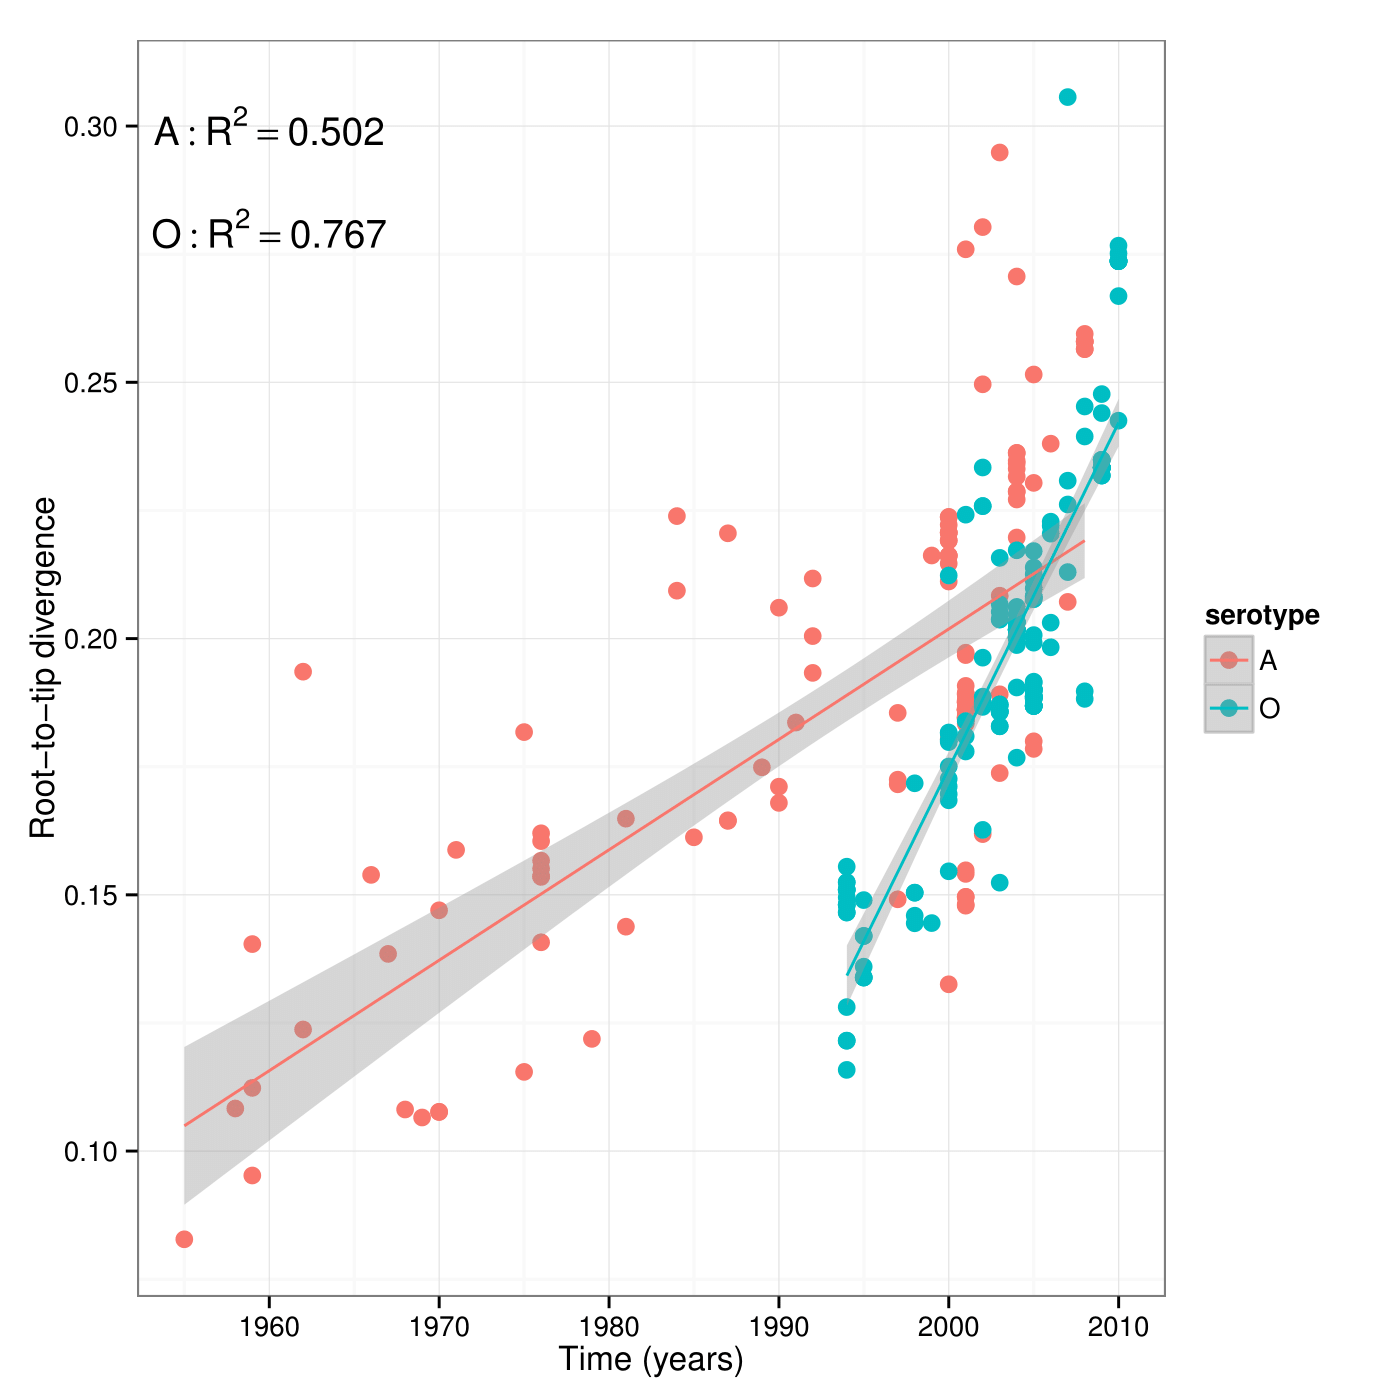
\includegraphics[scale=.35]{FIGURES/rdvs.png}
\end{center}
\caption{}
\label{sfig:root-to-tip}
\end{figure}
\end{center}
%%%%%%%%%%%%%%%%%%
%%%%%%%%%%%%%%%%%%
\newpage
\begin{center}
\begin{figure}[H]
\begin{center}
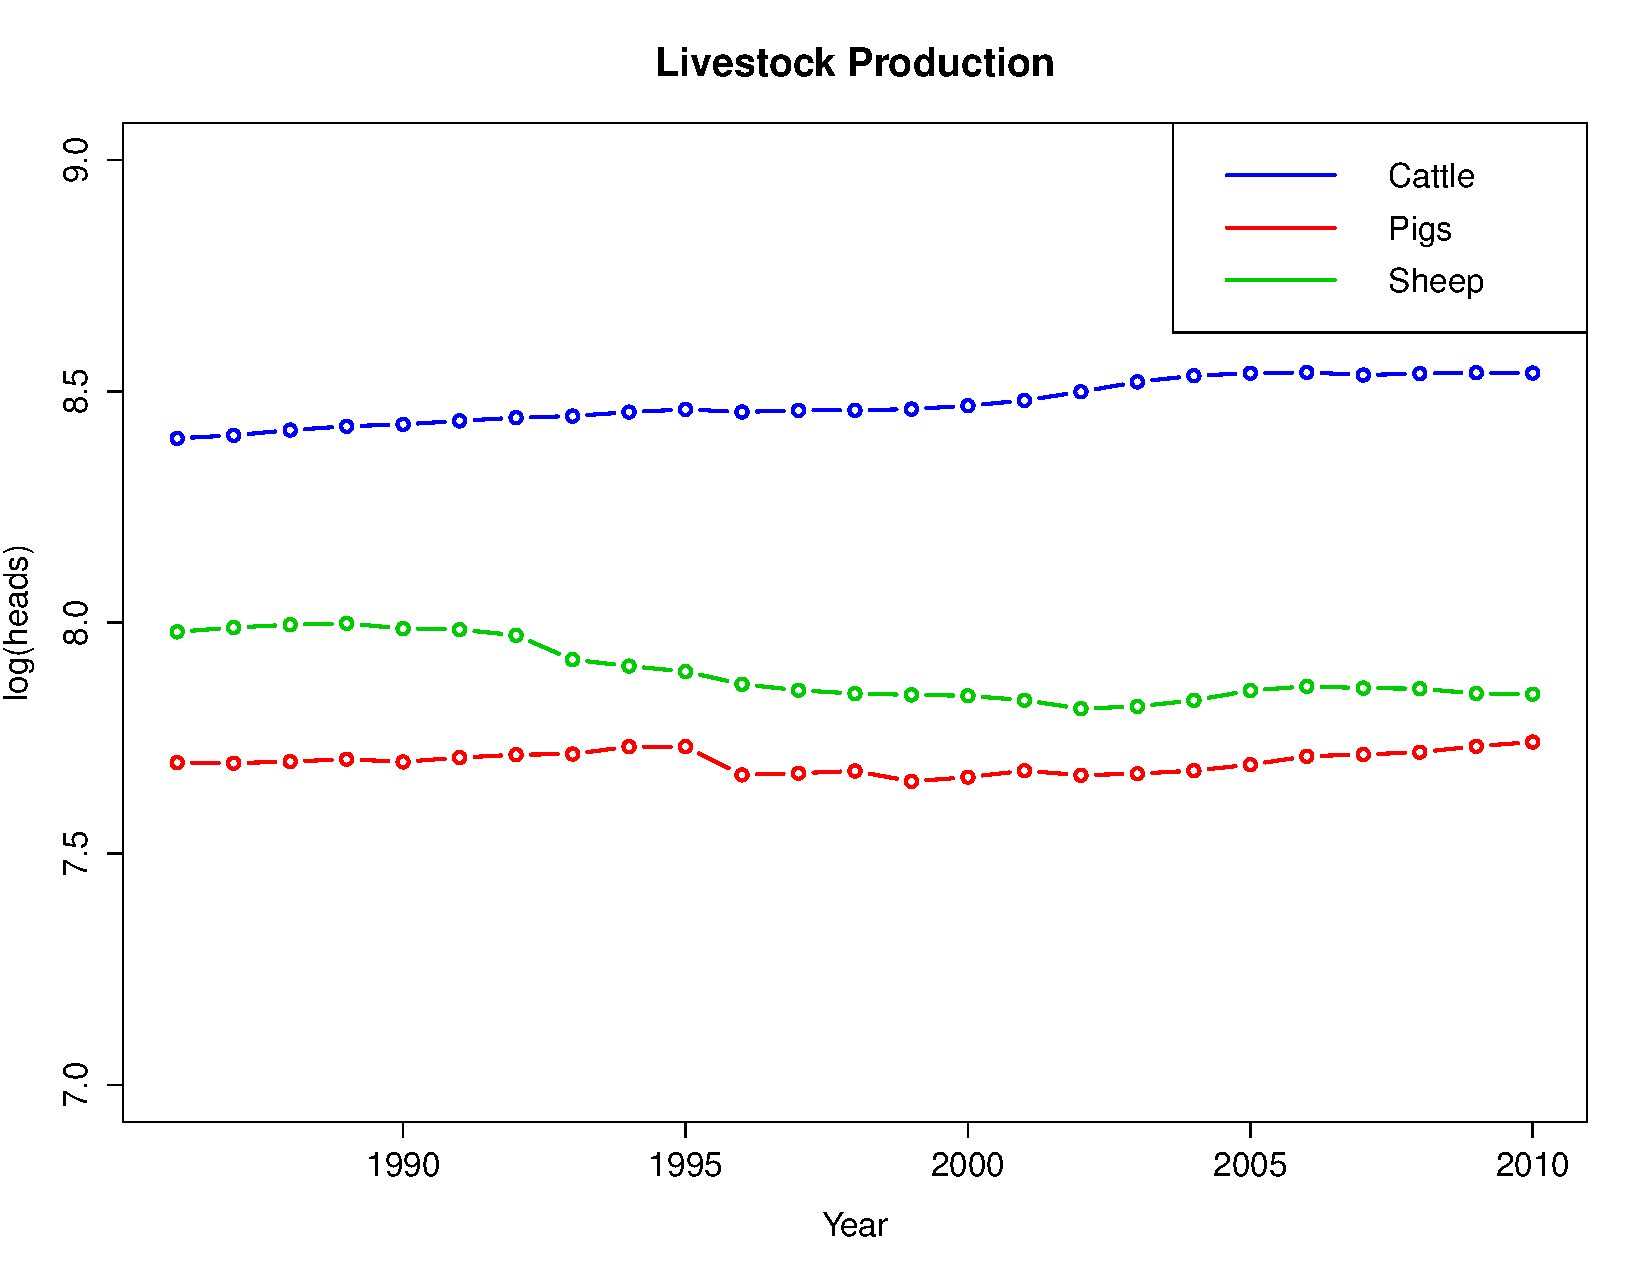
\includegraphics[scale=.80]{FIGURES/production.pdf}
\end{center}
\caption{}
\label{sfig:prod}
\end{figure}
\end{center}
%%%%%%%%%%%%%%%%%%%
%%%%%%%%%%%%%%%%%%%
\newpage
\begin{center}
\begin{figure}[H]
\begin{center}
\subfigure[]{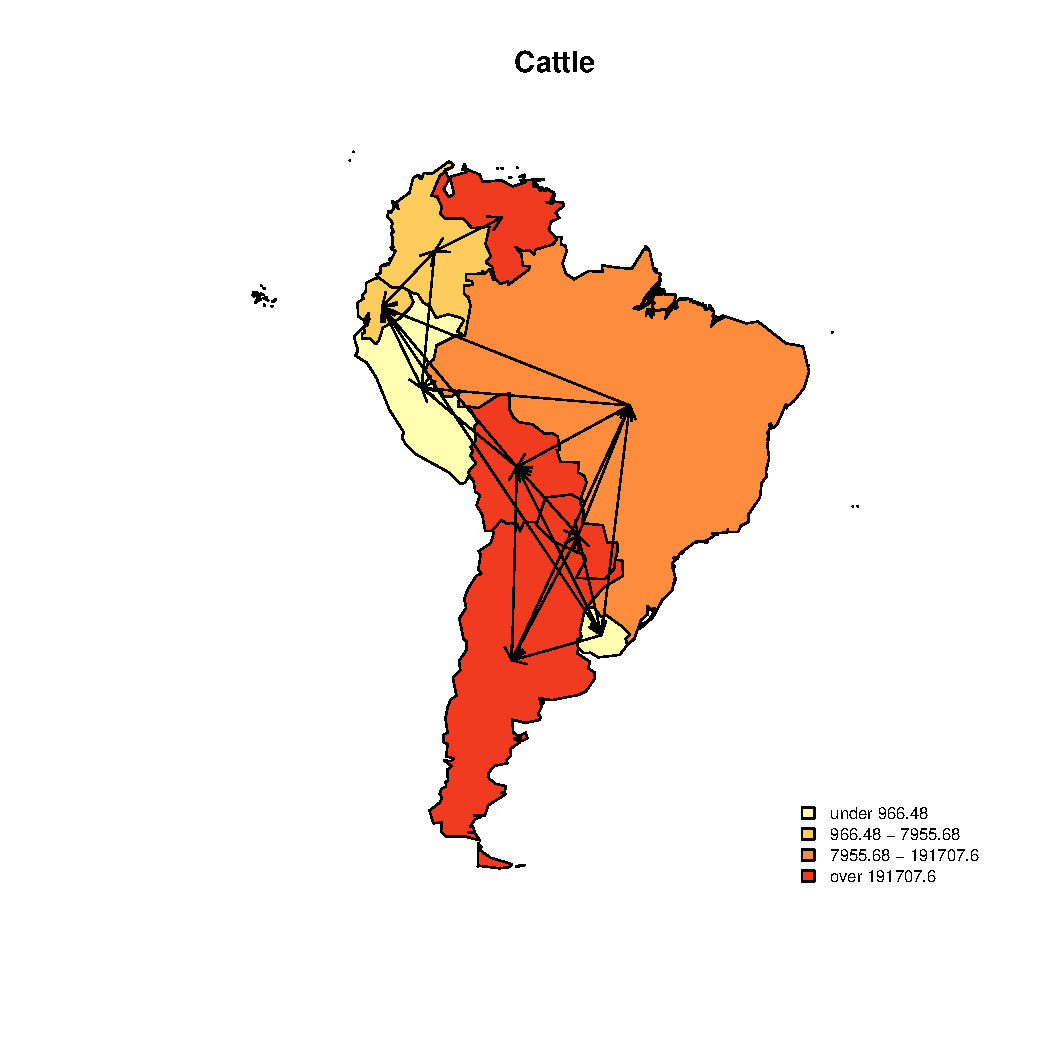
\includegraphics[scale=.400]{FIGURES/tradenets_cattle_s=0.pdf}}
\subfigure[]{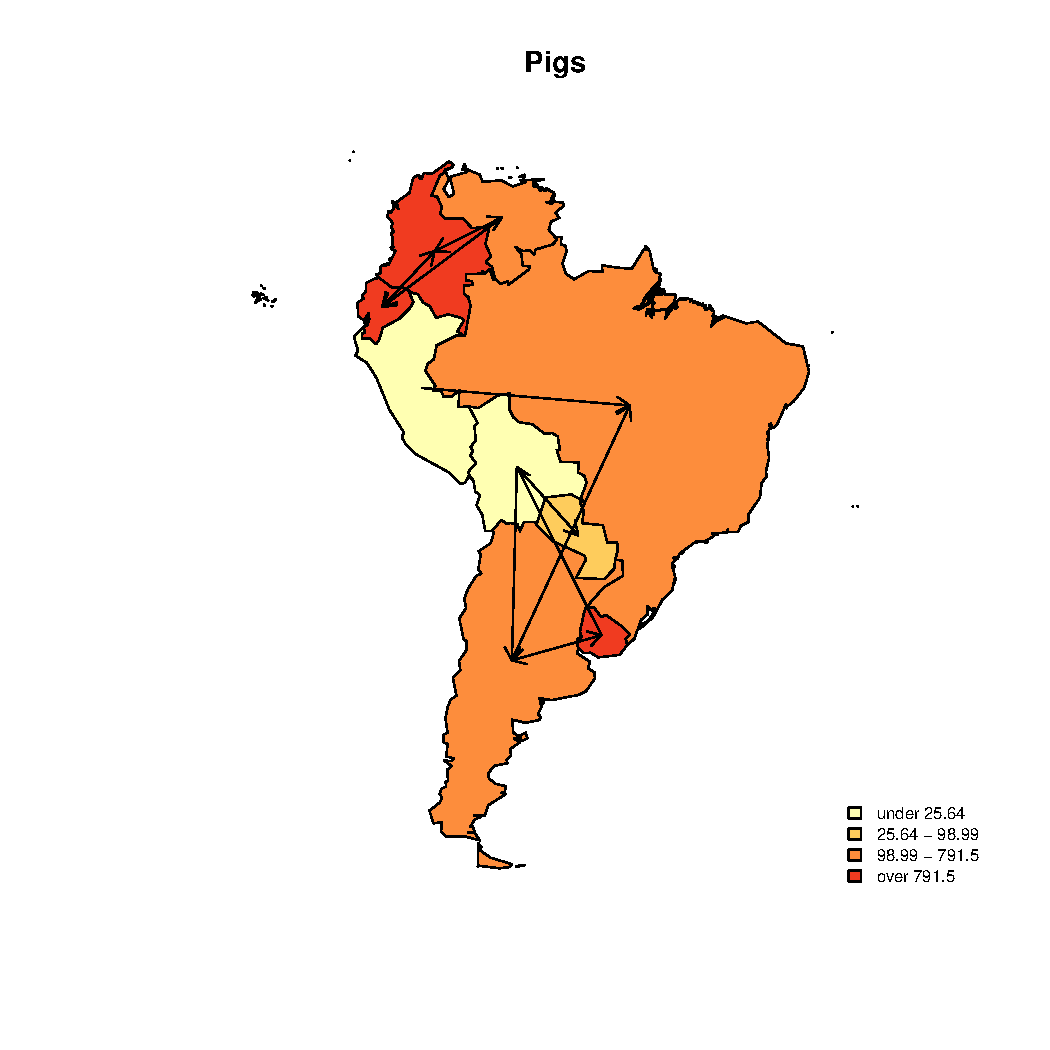
\includegraphics[scale=.400]{FIGURES/tradenets_pig_s=0.pdf}} \\
\subfigure[]{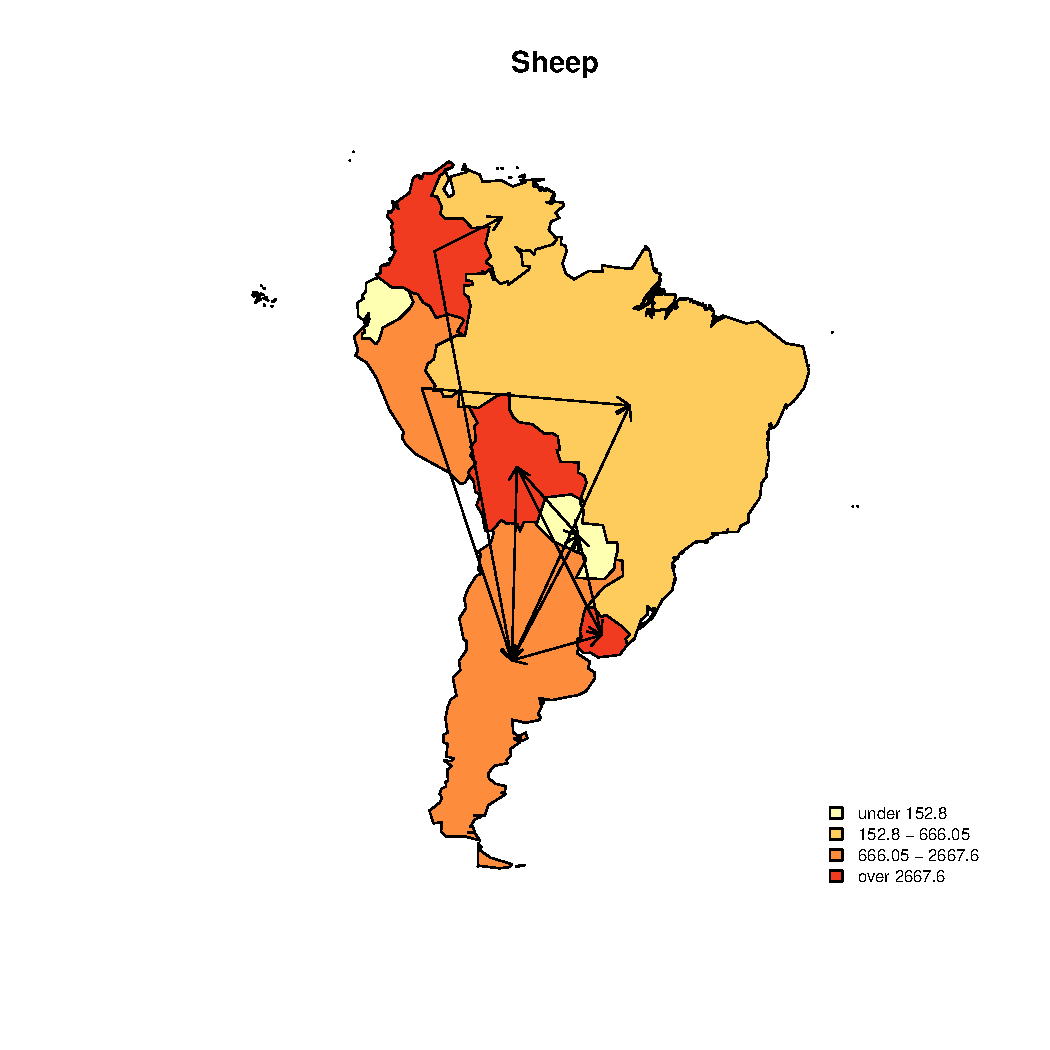
\includegraphics[scale=.400]{FIGURES/tradenets_sheep_s=0.pdf}}
\end{center}
\caption{}
\label{sfig:tradenets}
\end{figure}
\end{center}
%%%%%%%%%%%%%%%%
%%%%%%%%%%%%%%%%
\newpage
\begin{figure}[H]
\begin{center}
\subfigure[]{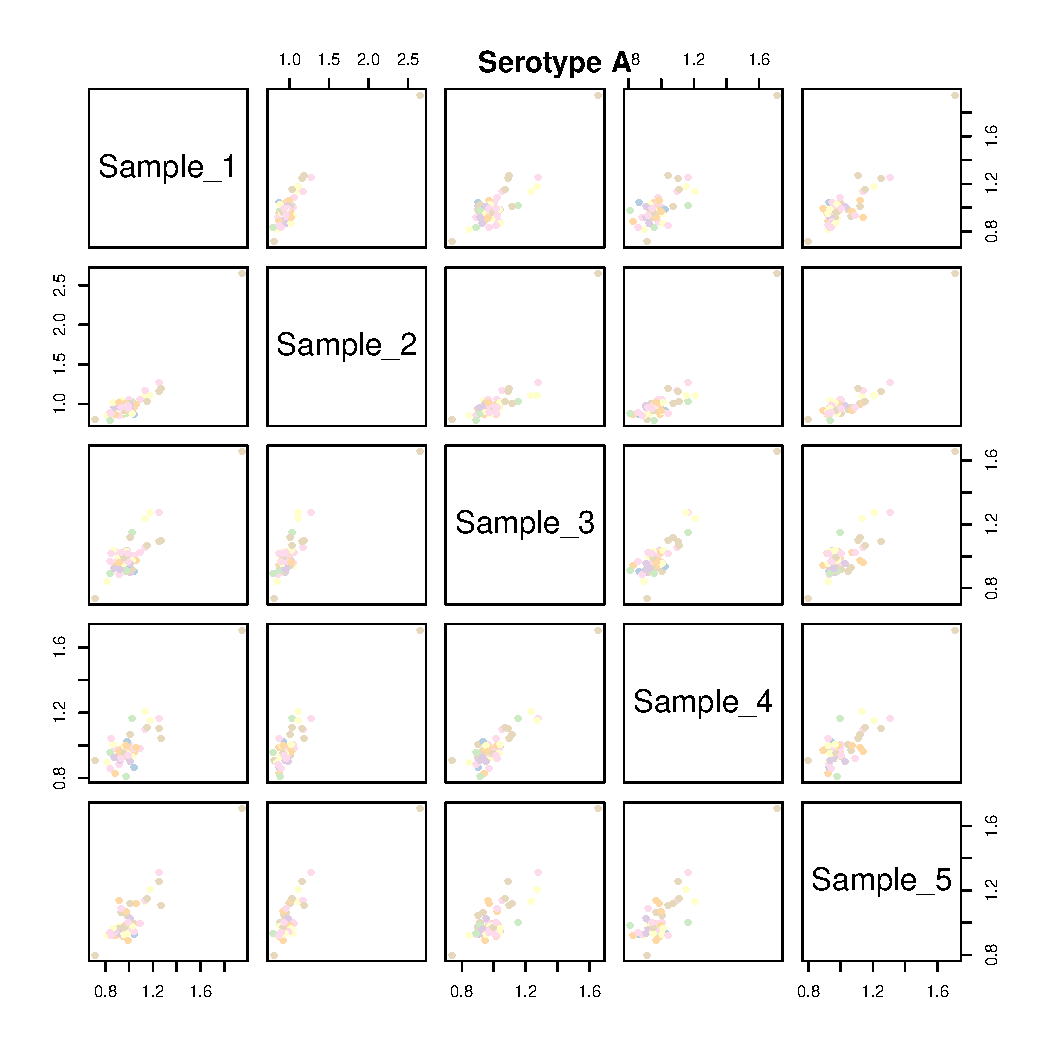
\includegraphics[scale=.400]{FIGURES/rateplotA.pdf}}
\subfigure[]{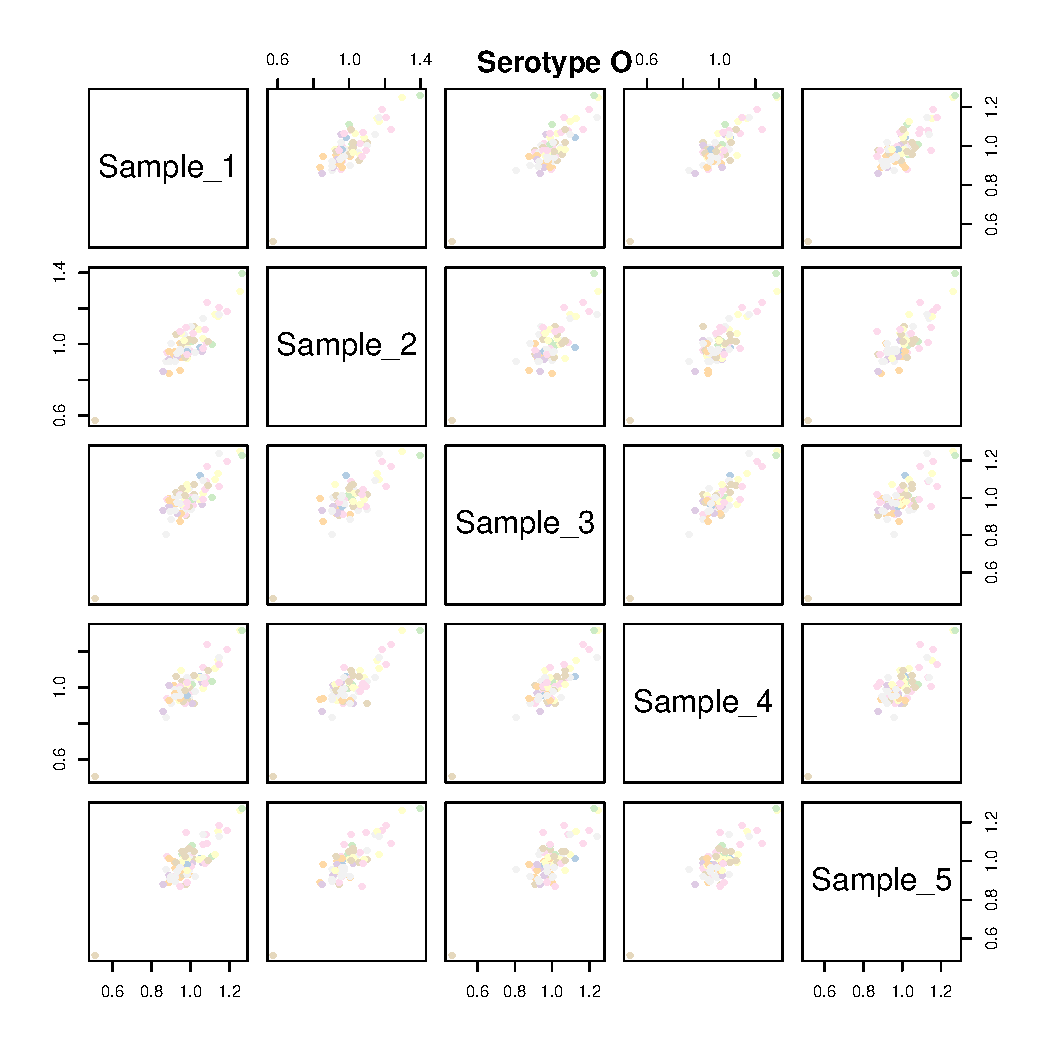
\includegraphics[scale=.400]{FIGURES/rateplotO.pdf}}\\
\subfigure[]{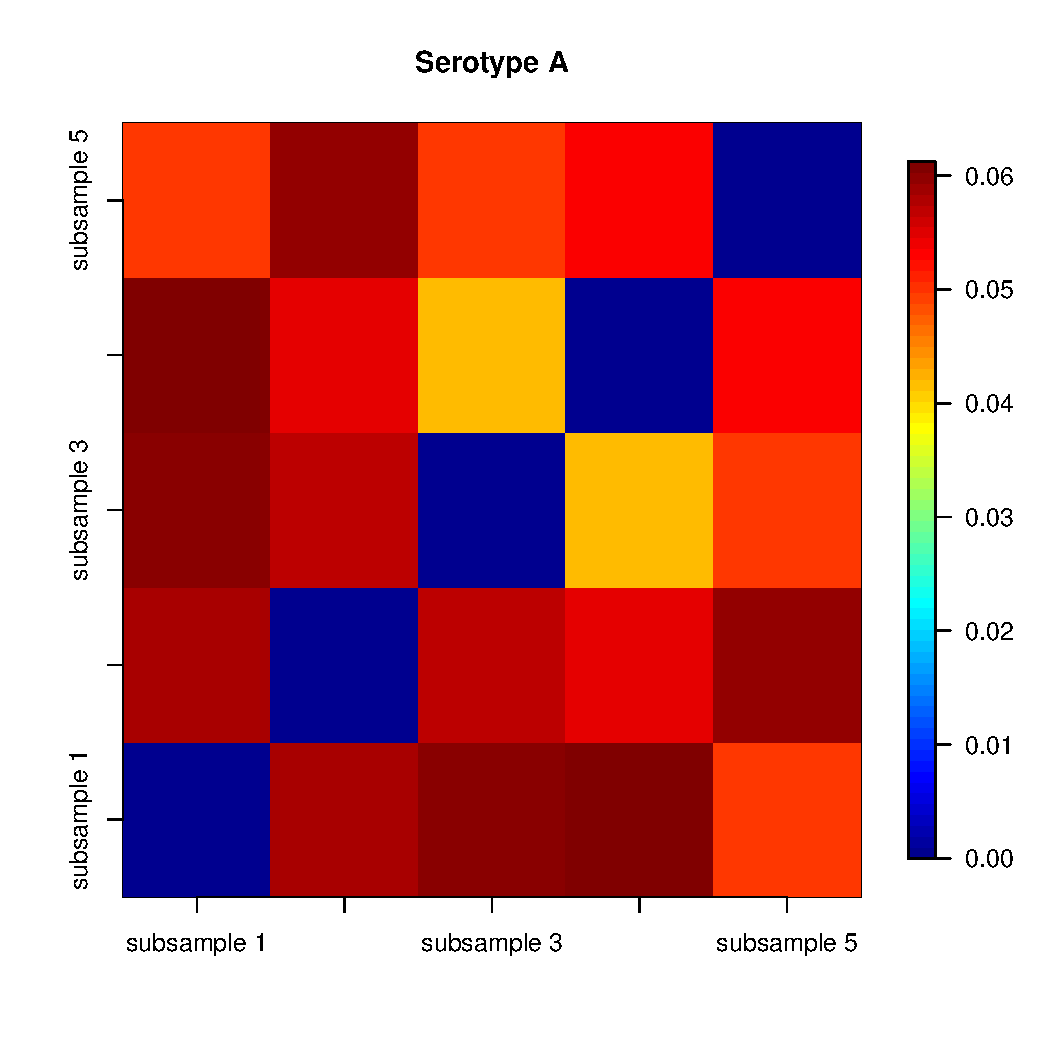
\includegraphics[scale=.400]{FIGURES/normplotA.pdf}}
\subfigure[]{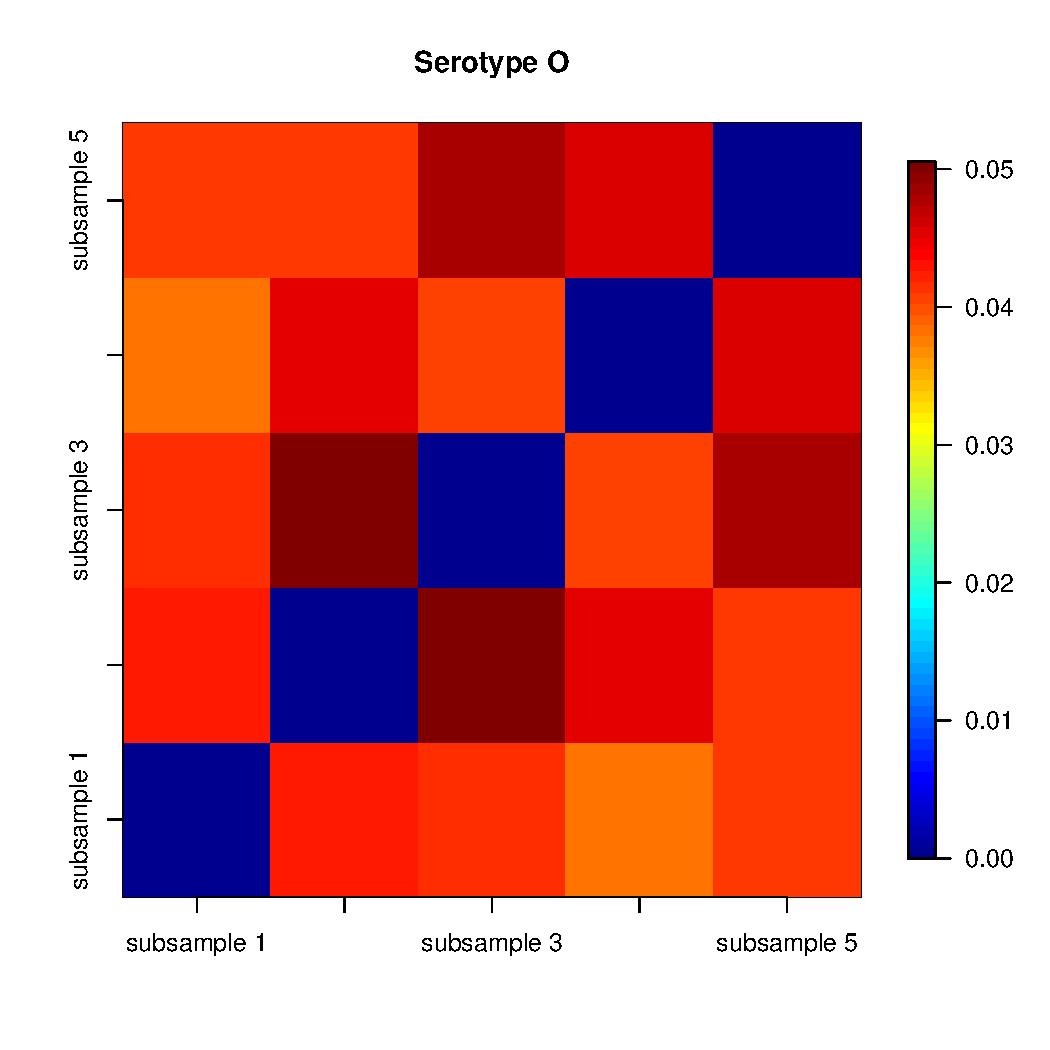
\includegraphics[scale=.400]{FIGURES/normplotO.pdf}}
\end{center}
\caption{}
\label{sfig:compz}
\end{figure}
%%%%%%%%%%%%%%%%
%%%%%%%%%%%%%%%%
\newpage
\begin{center}
\begin{figure}[H]
\begin{center}
\subfigure[]{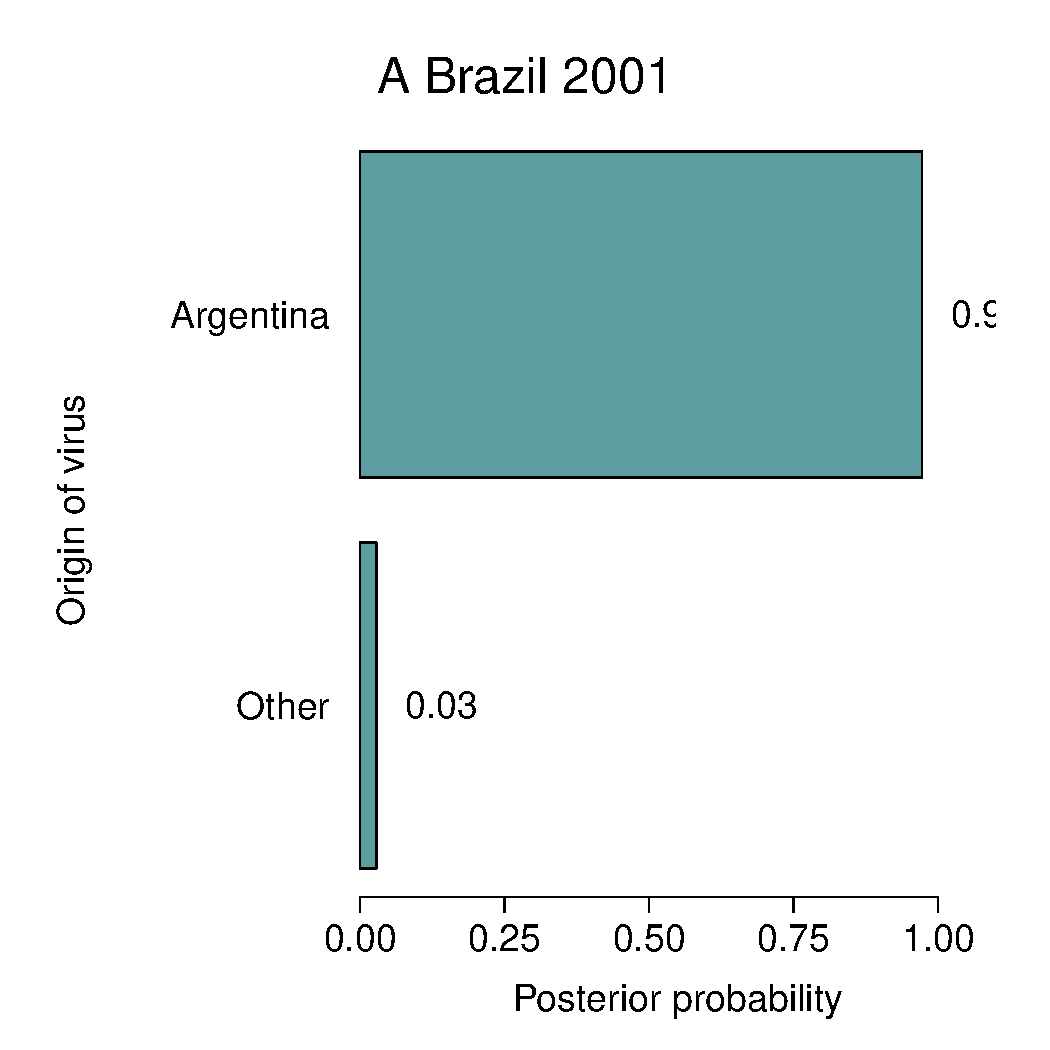
\includegraphics[scale=.40]{FIGURES/Origins_A_Brazil_2001.pdf}}
\subfigure[]{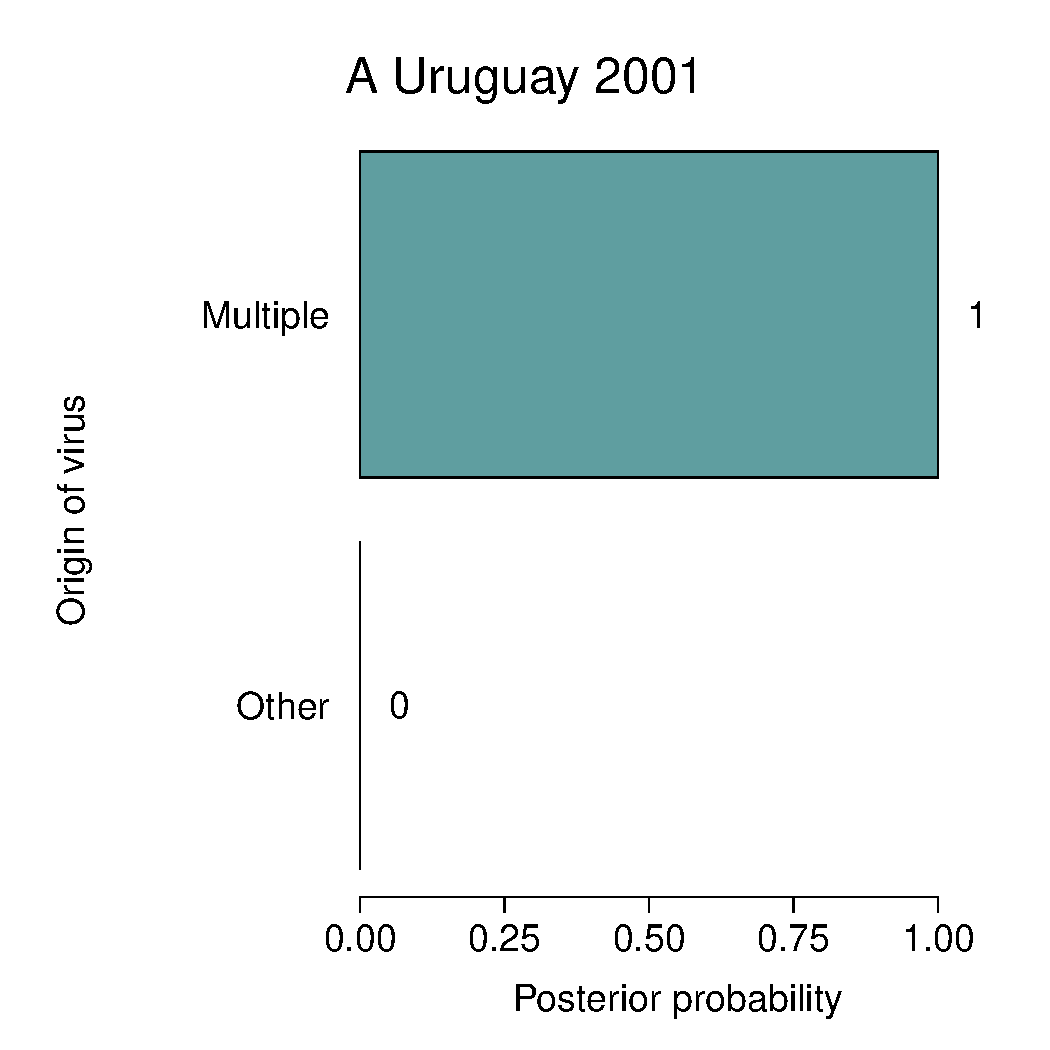
\includegraphics[scale=.40]{FIGURES/Origins_A_Uruguay_2001.pdf}}\\
\subfigure[]{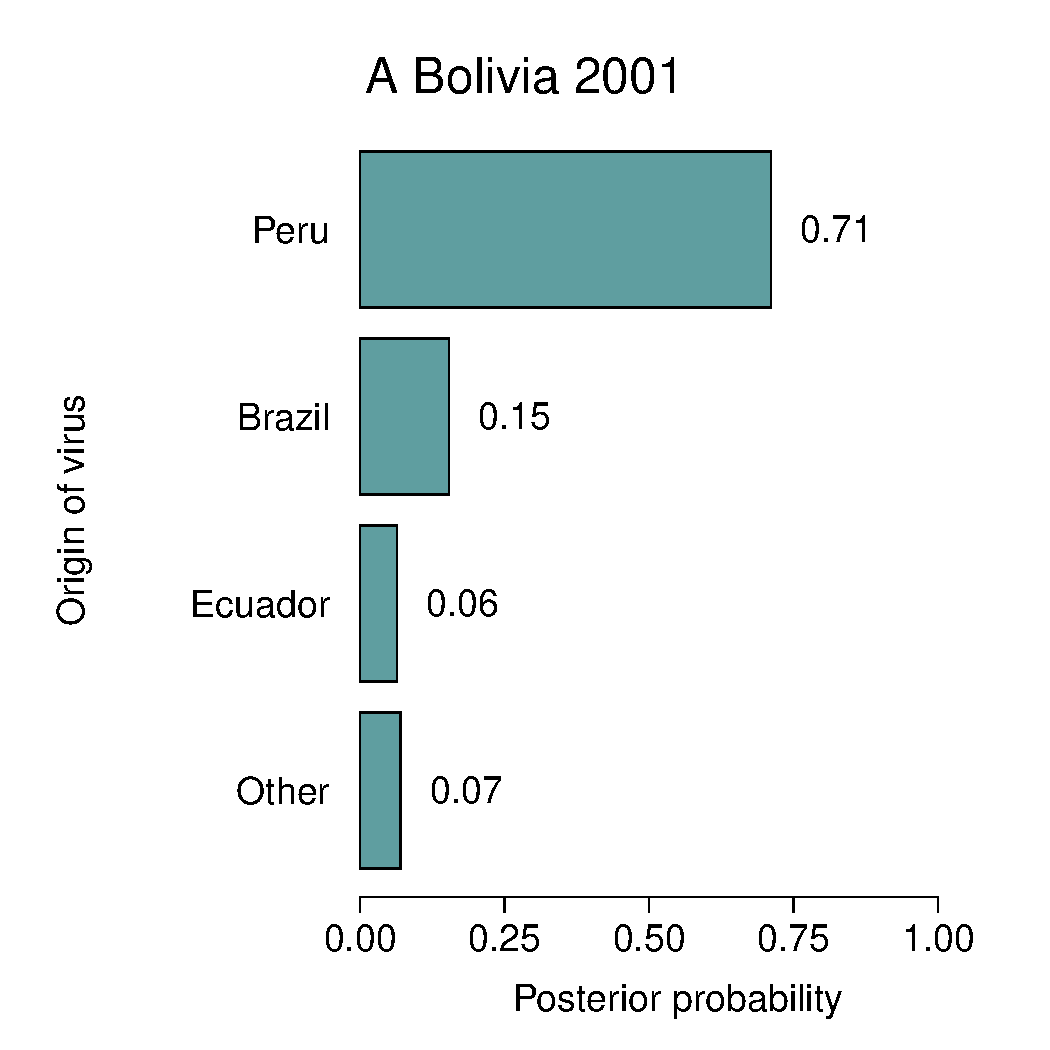
\includegraphics[scale=.40]{FIGURES/Origins_A_Bolivia_2001.pdf}}
\subfigure[]{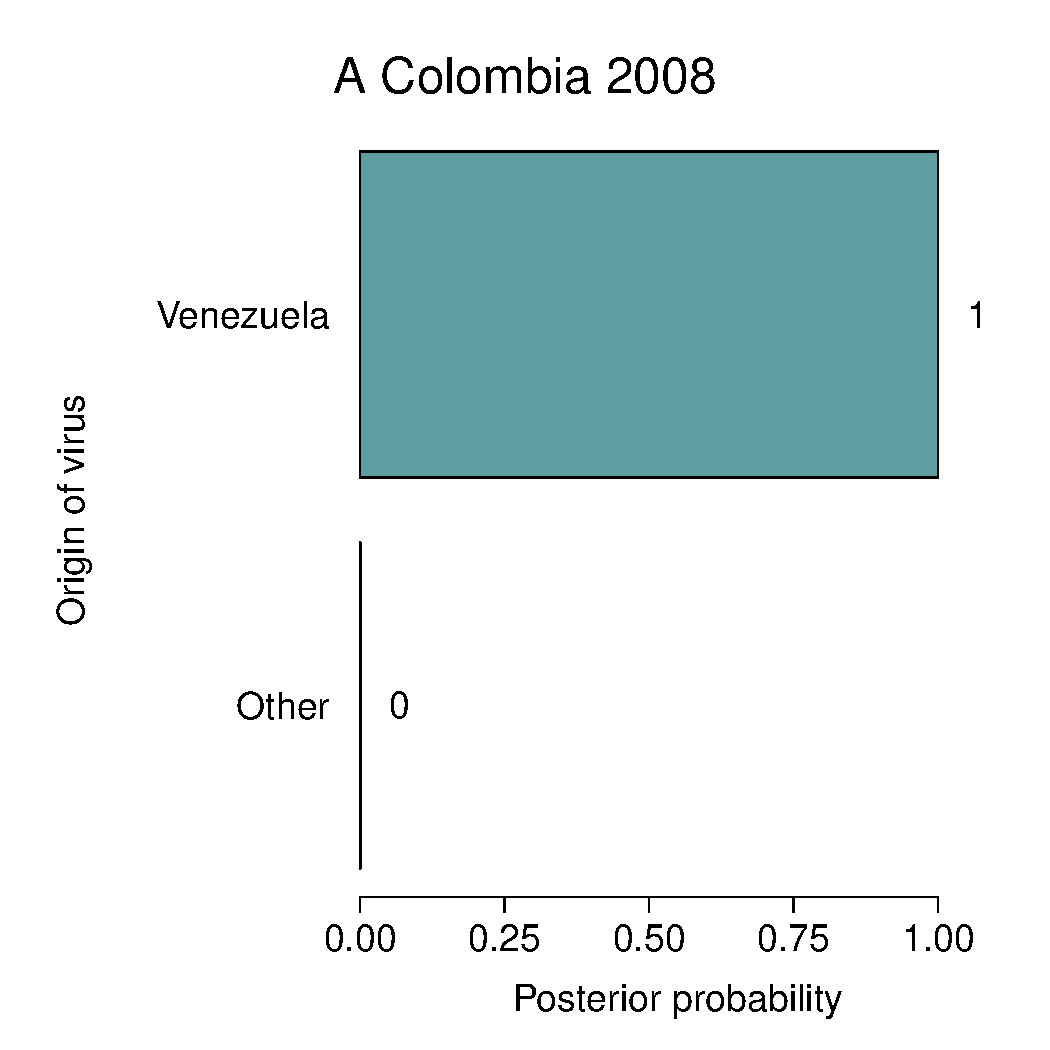
\includegraphics[scale=.40]{FIGURES/Origins_A_Colombia_2008.pdf}}\\
\subfigure[]{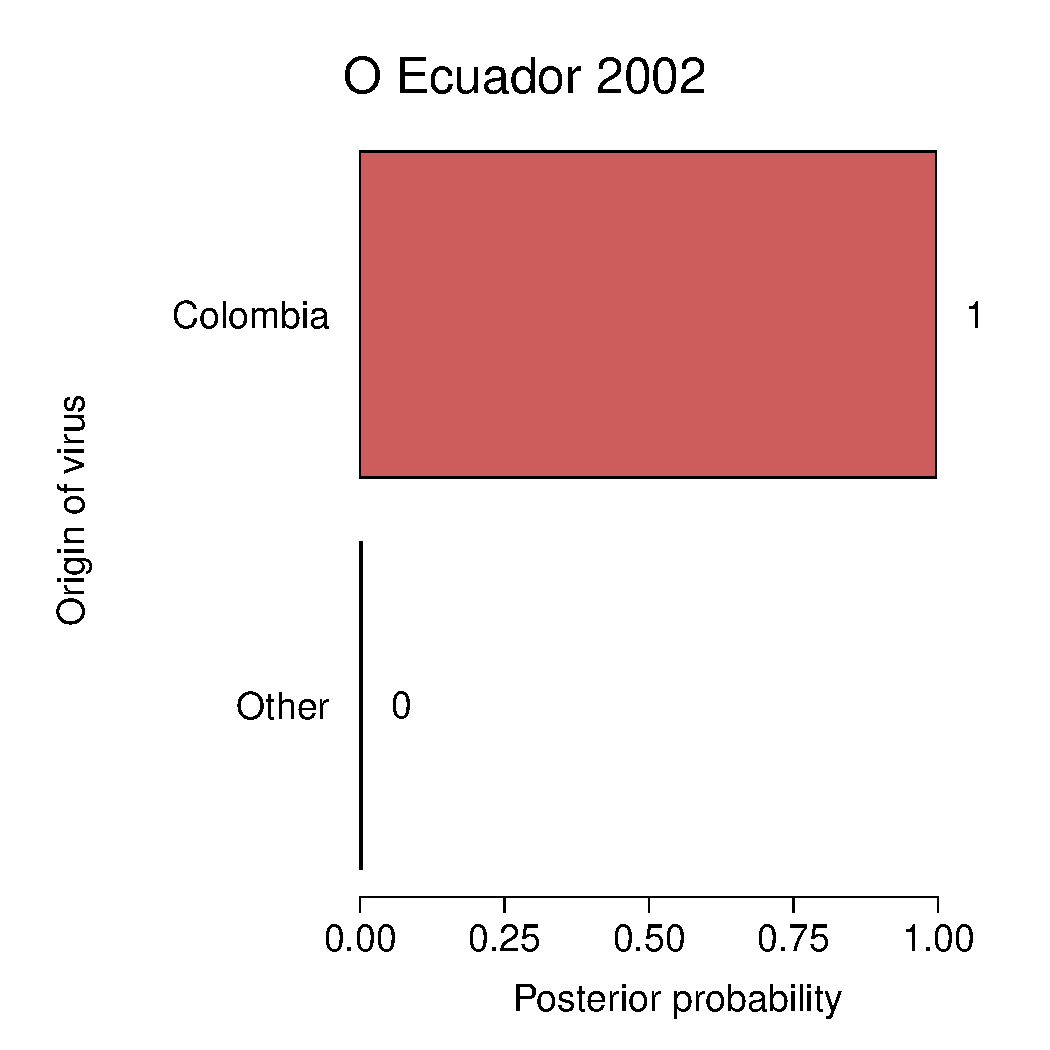
\includegraphics[scale=.40]{FIGURES/Origins_O_Ecuador_2002.pdf}}
\subfigure[]{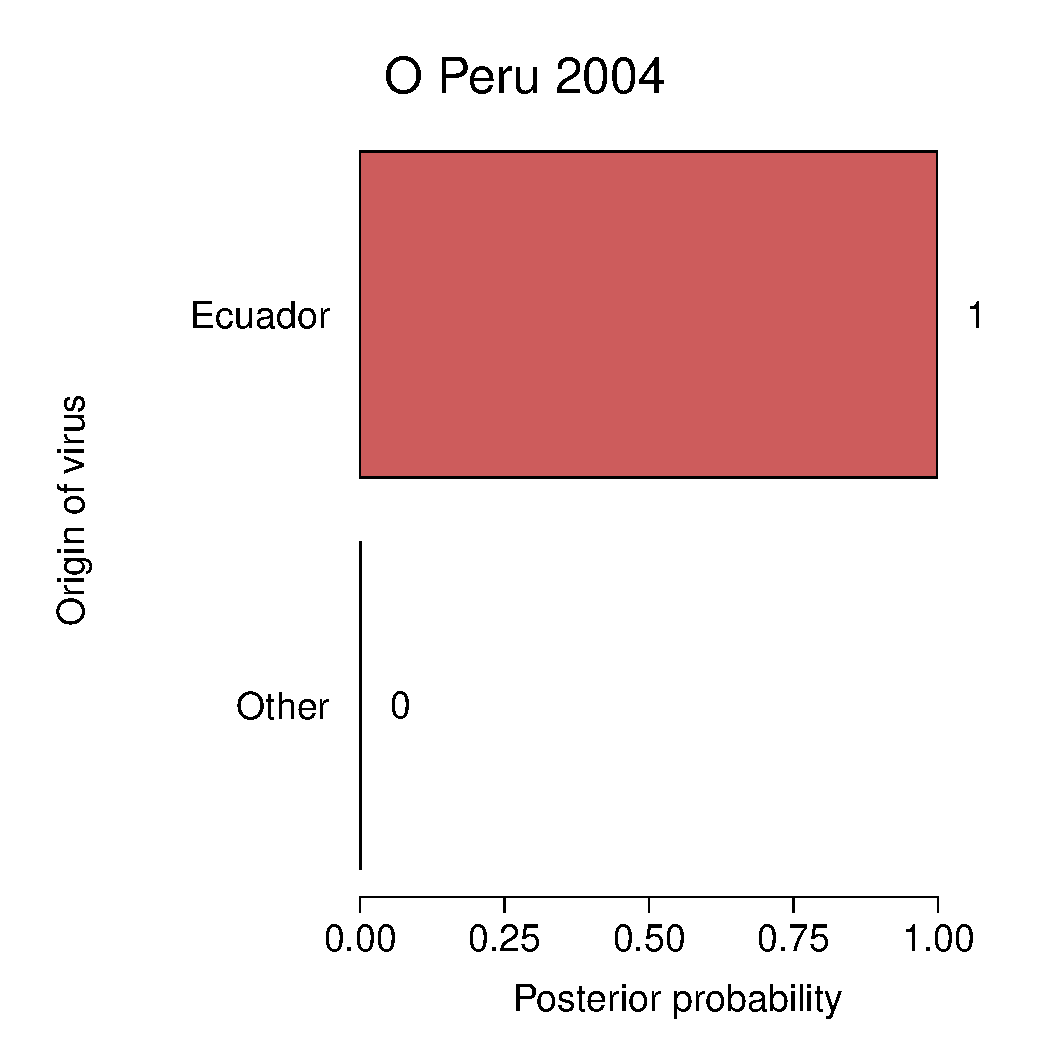
\includegraphics[scale=.40]{FIGURES/Origins_O_Peru_2004.pdf}}
\end{center}
\caption{}
\label{sfig:epitrac}
\end{figure}
\end{center}
%%%%%%%%%%%%%%%%%%%
%%%%%%%%%%%%%%%%%%%
\newpage
\begin{figure}[H]
\begin{center}
\subfigure[]{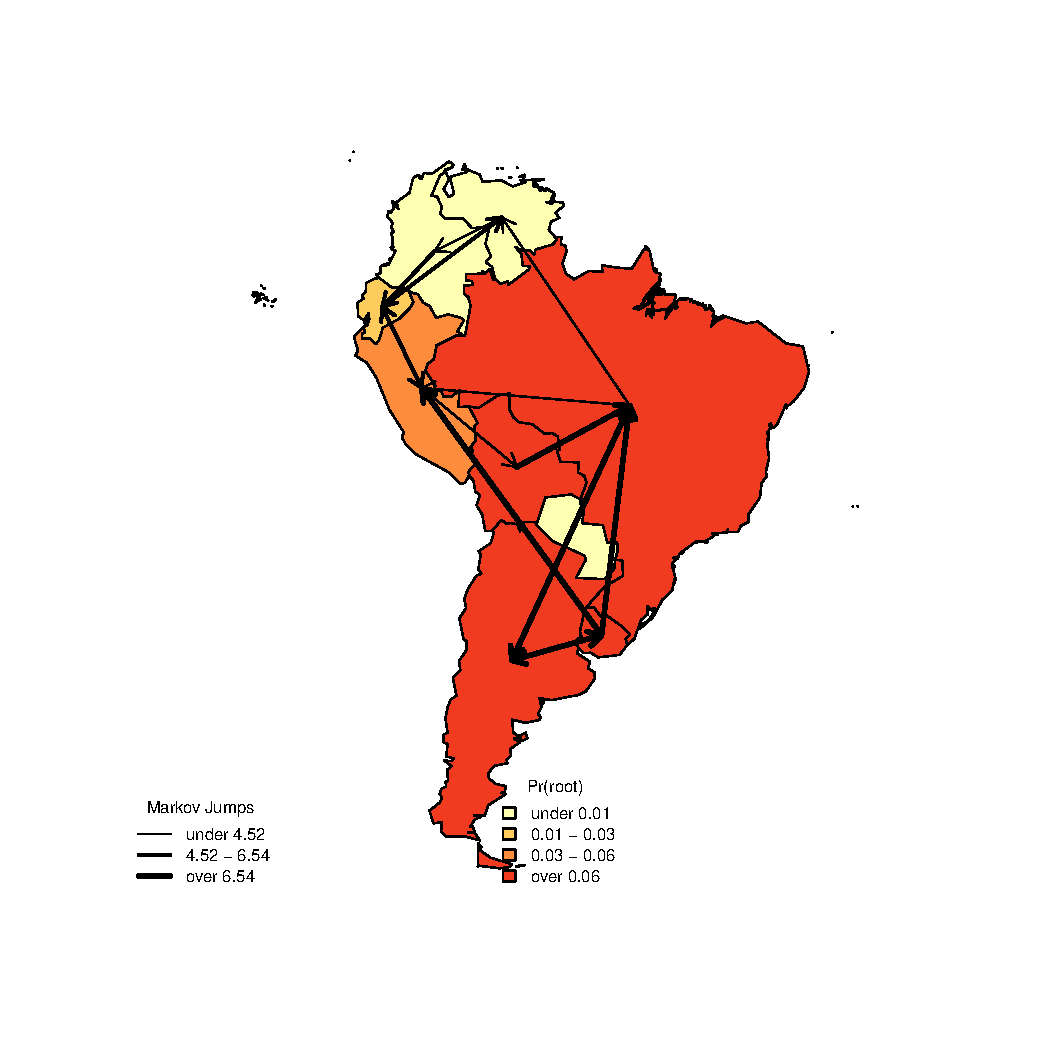
\includegraphics[scale=.350]{FIGURES/A_ss1.pdf}}
\subfigure[]{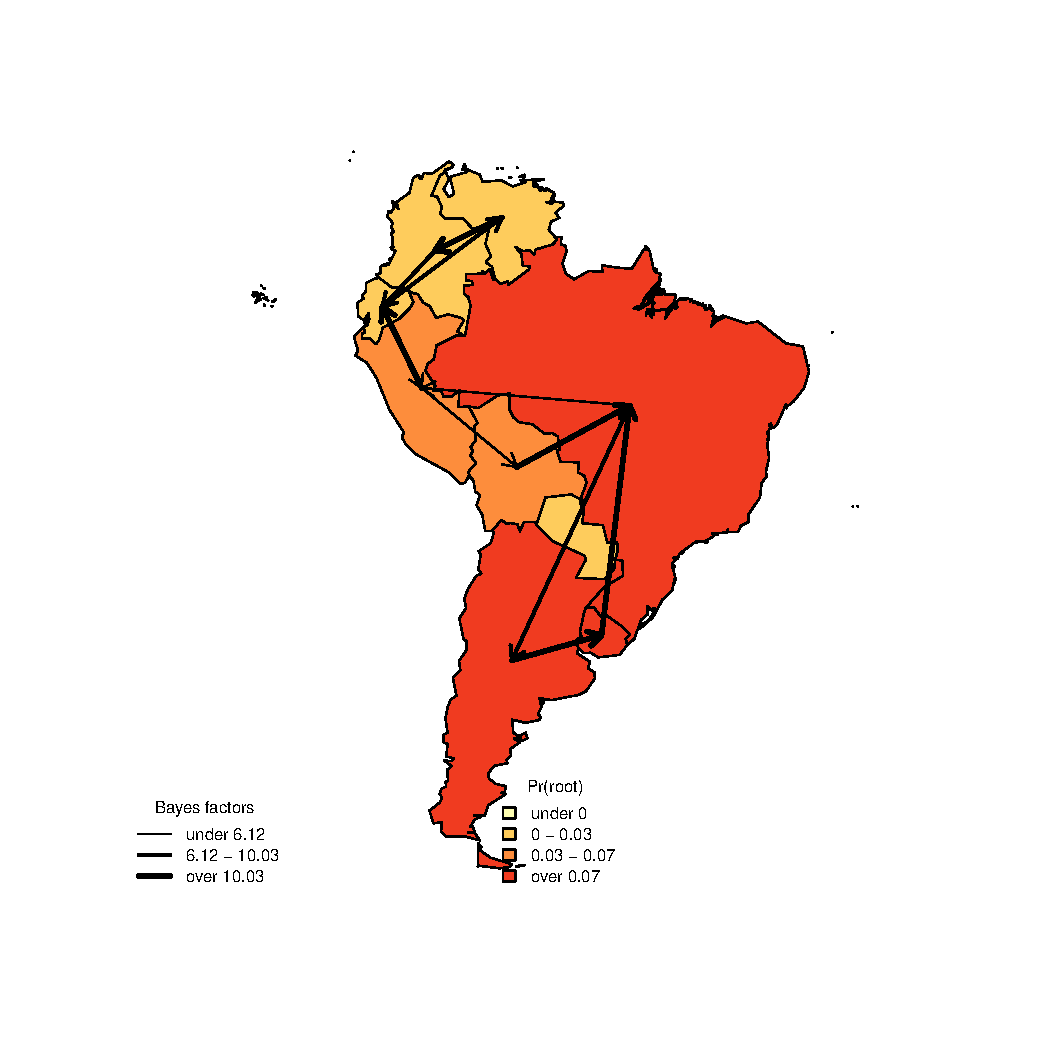
\includegraphics[scale=.350]{FIGURES/A_ss2.pdf}}\\
\subfigure[]{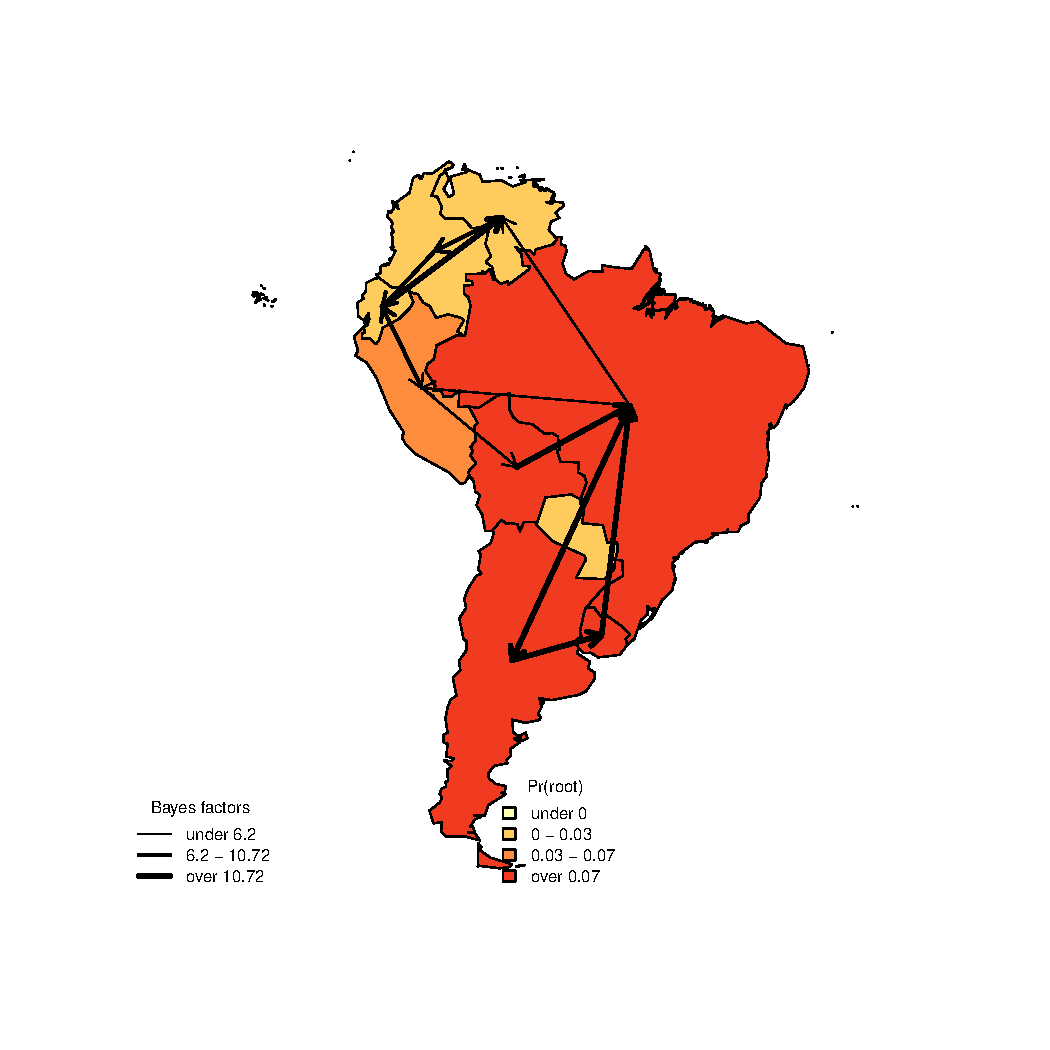
\includegraphics[scale=.350]{FIGURES/A_ss3.pdf}}
\subfigure[]{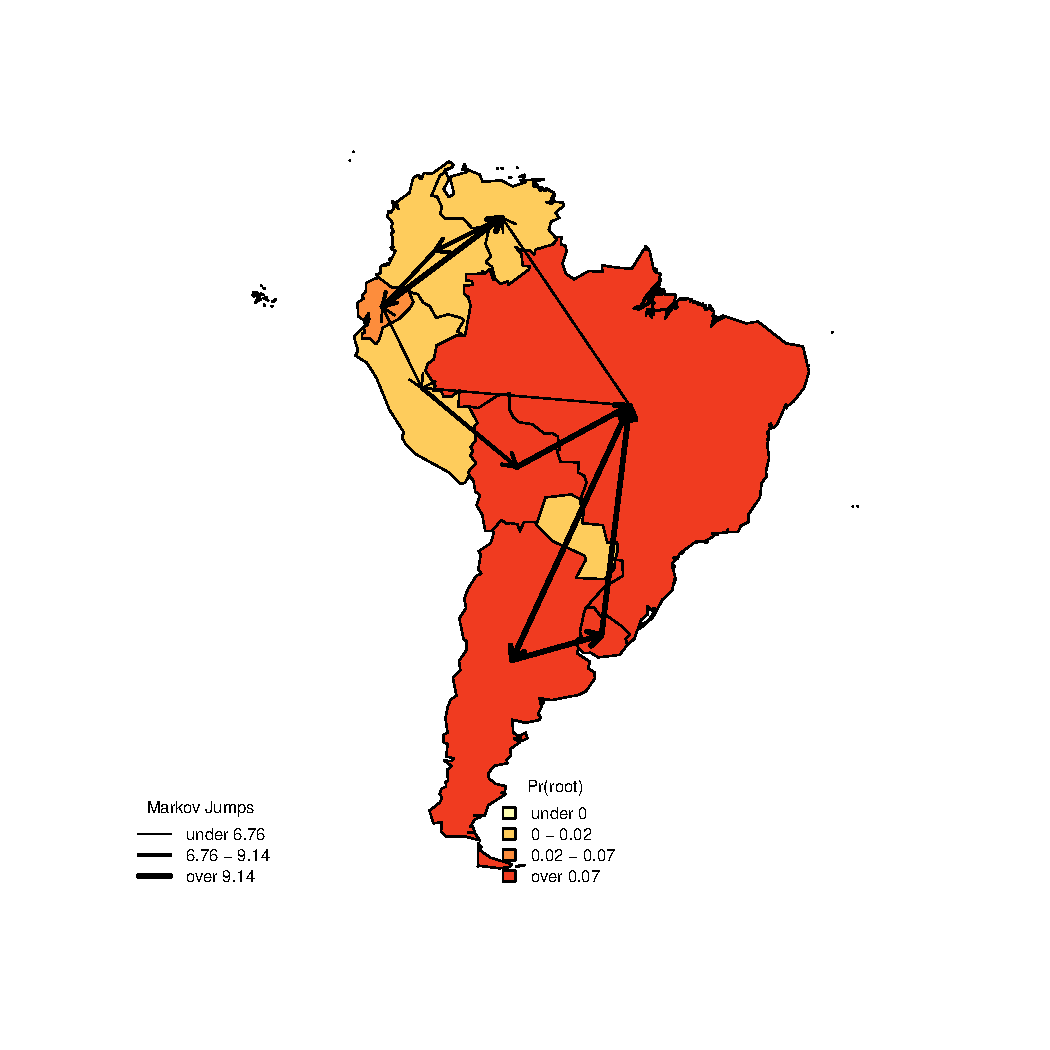
\includegraphics[scale=.350]{FIGURES/A_ss4.pdf}}\\
\subfigure[]{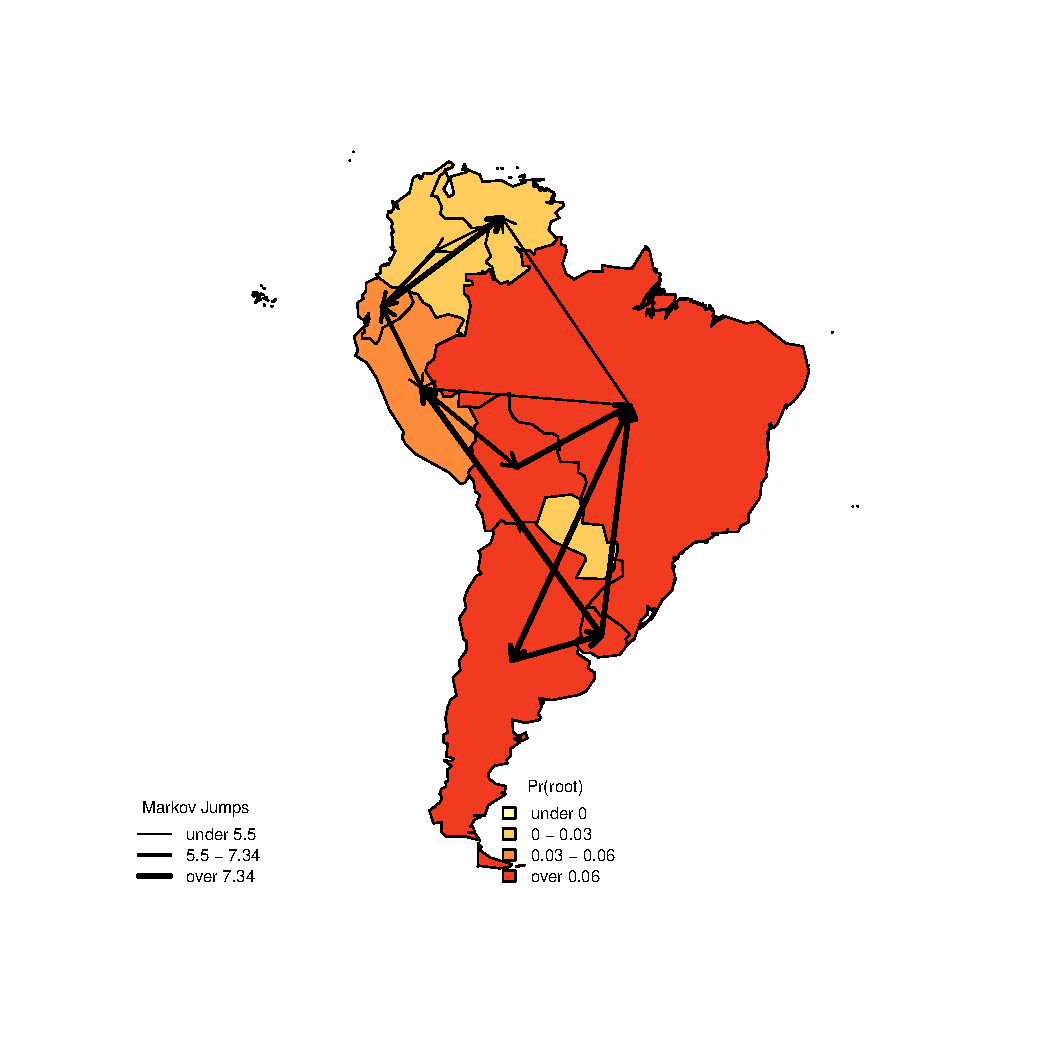
\includegraphics[scale=.350]{FIGURES/A_ss5.pdf}}
\caption{}
\label{sfig:bssvsA}
\end{center}
\end{figure}
%%%%%%%%%%%%%%%
%%%%%%%%%%%%%%%
\newpage
\begin{figure}[H]
\begin{center}
\subfigure[]{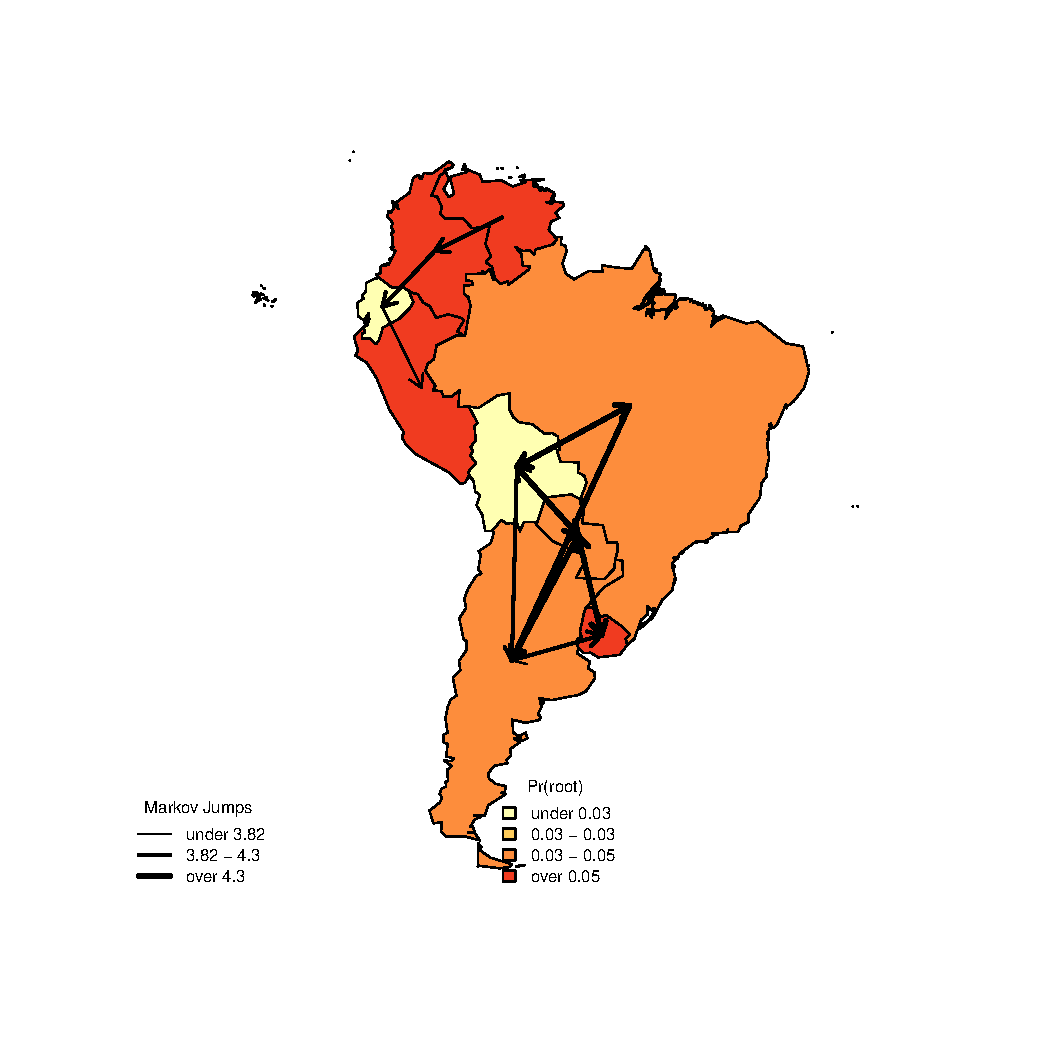
\includegraphics[scale=.350]{FIGURES/O_ss1.pdf}}
\subfigure[]{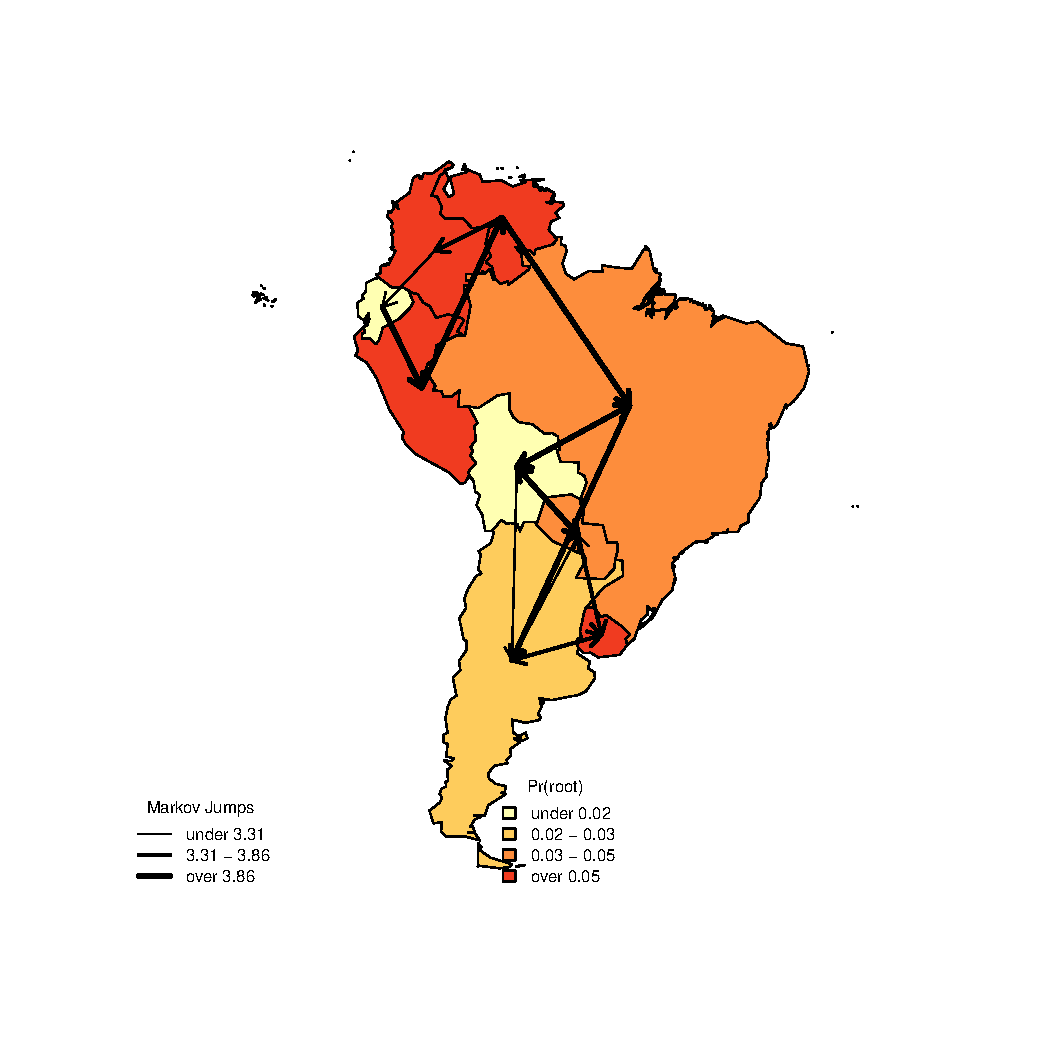
\includegraphics[scale=.350]{FIGURES/O_ss2.pdf}}\\
\subfigure[]{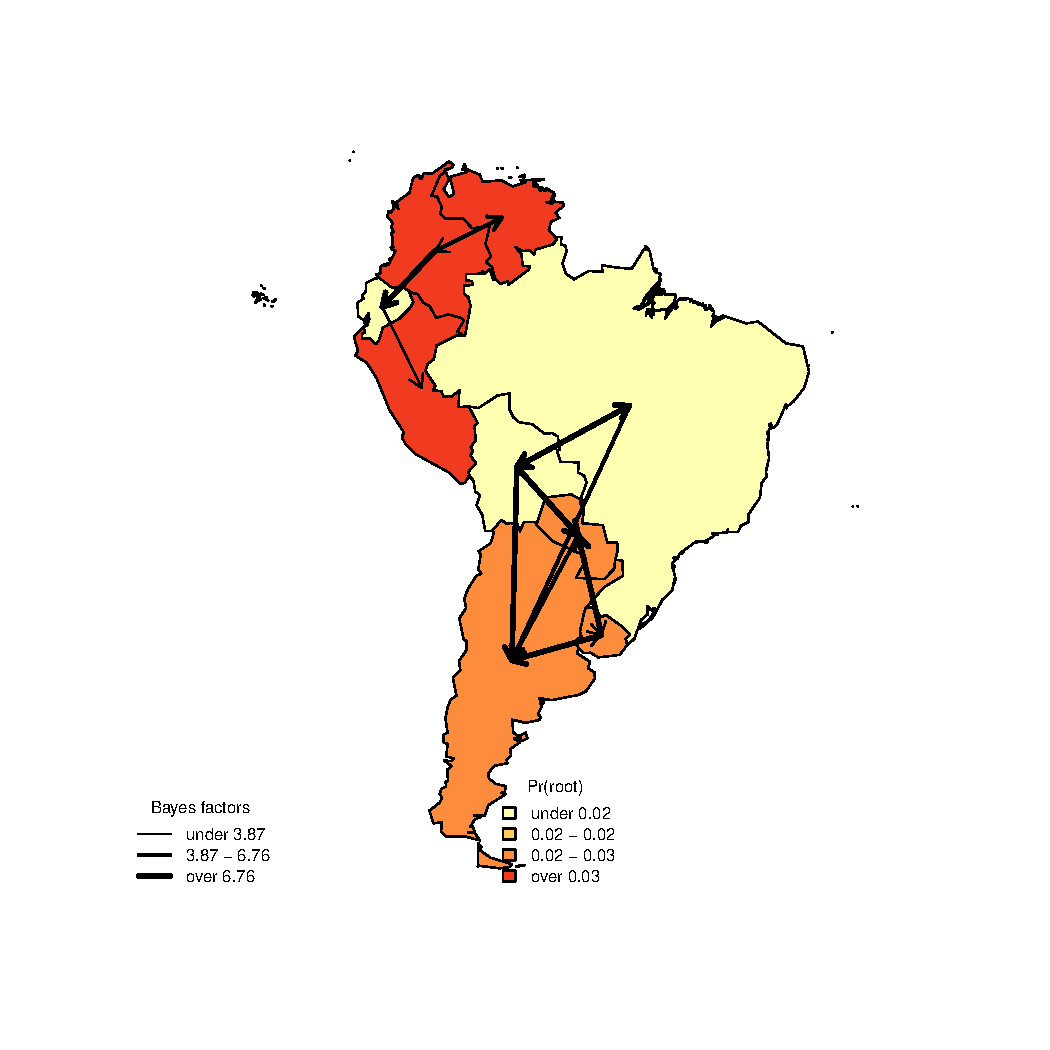
\includegraphics[scale=.350]{FIGURES/O_ss3.pdf}}
\subfigure[]{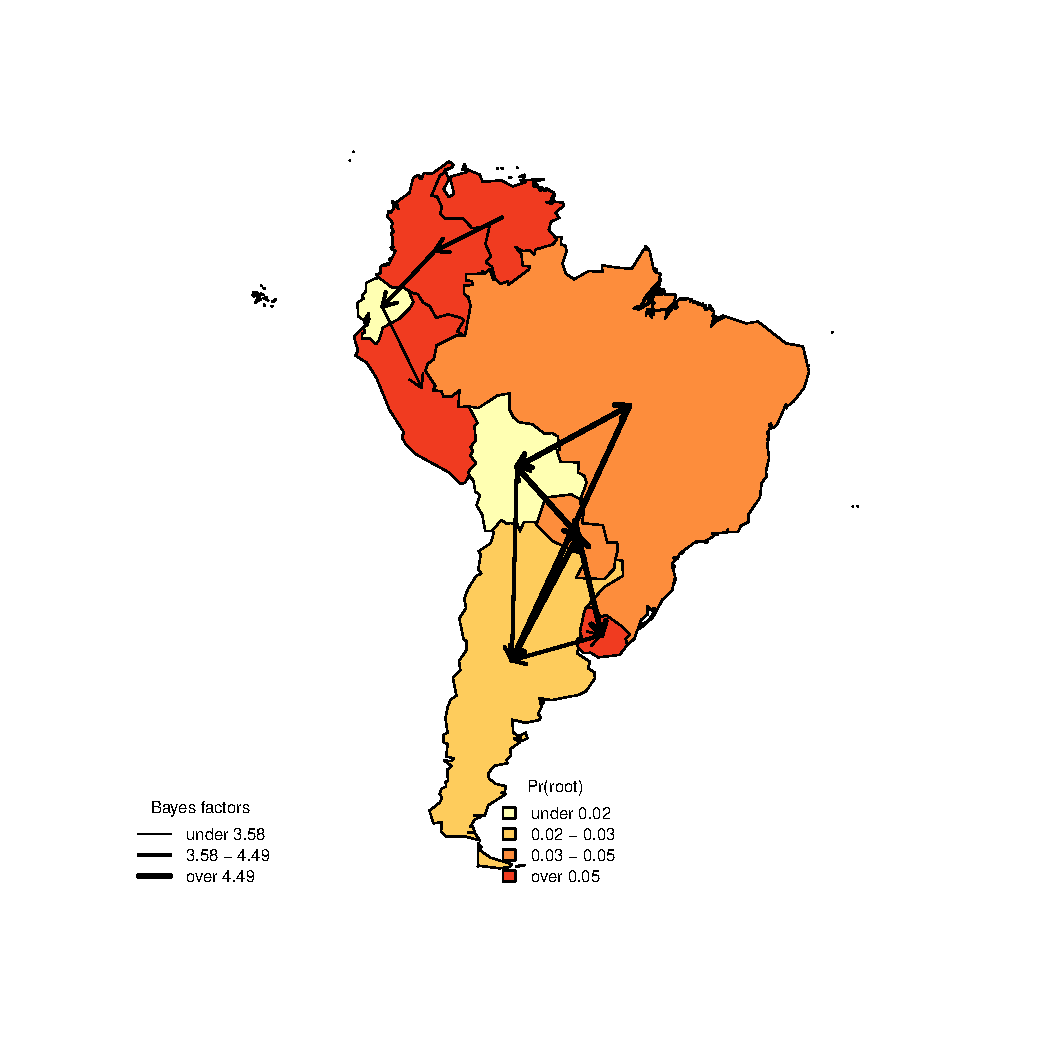
\includegraphics[scale=.350]{FIGURES/O_ss4.pdf}}\\
\subfigure[]{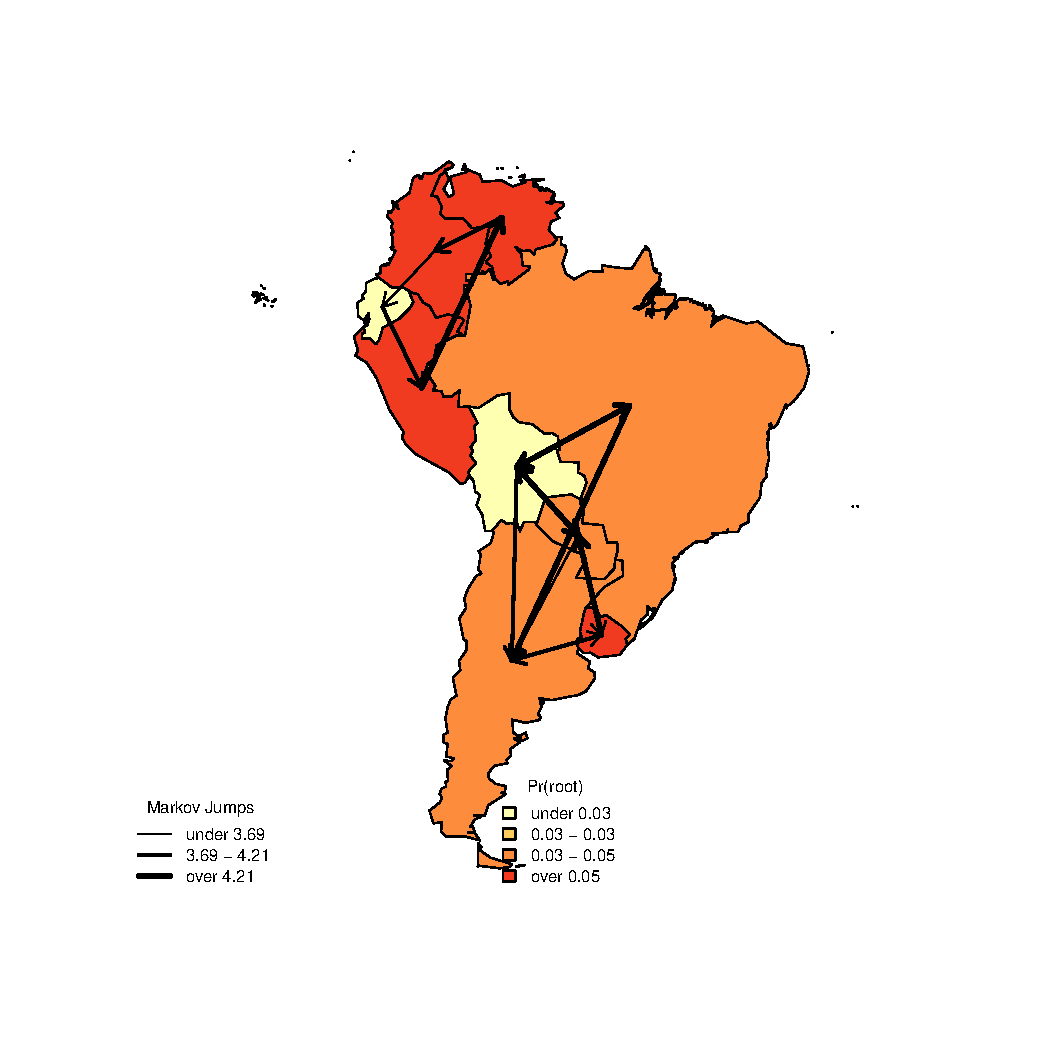
\includegraphics[scale=.350]{FIGURES/O_ss5.pdf}}
\end{center}
\caption{}
\label{sfig:bssvsO}
\end{figure}
%%%%%%%%%%%%%%%%
%%%%%%%%%%%%%%%%
\newpage
\begin{figure}[H]
\begin{center}
\subfigure[]{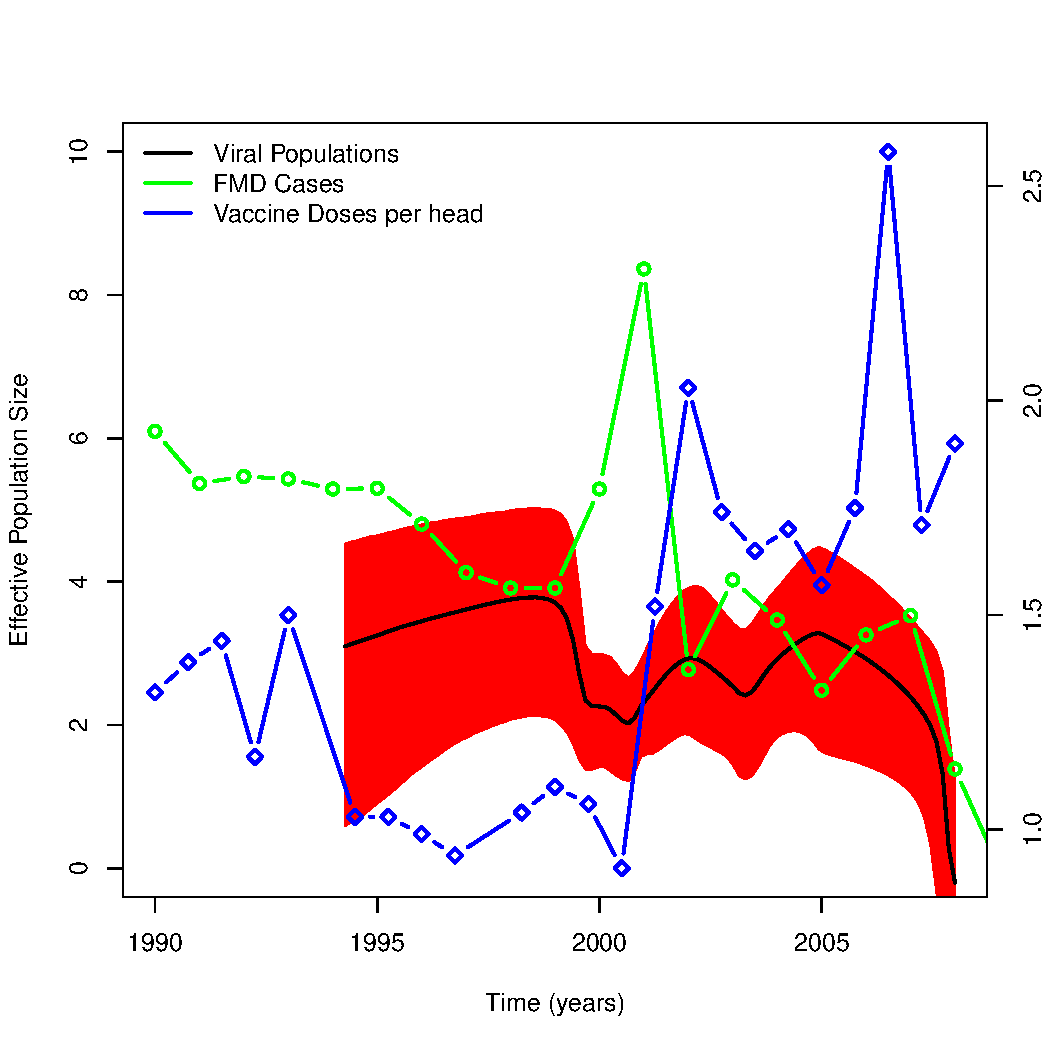
\includegraphics[scale=.60]{FIGURES/SFig_A2000sky.pdf}}\\
\subfigure[]{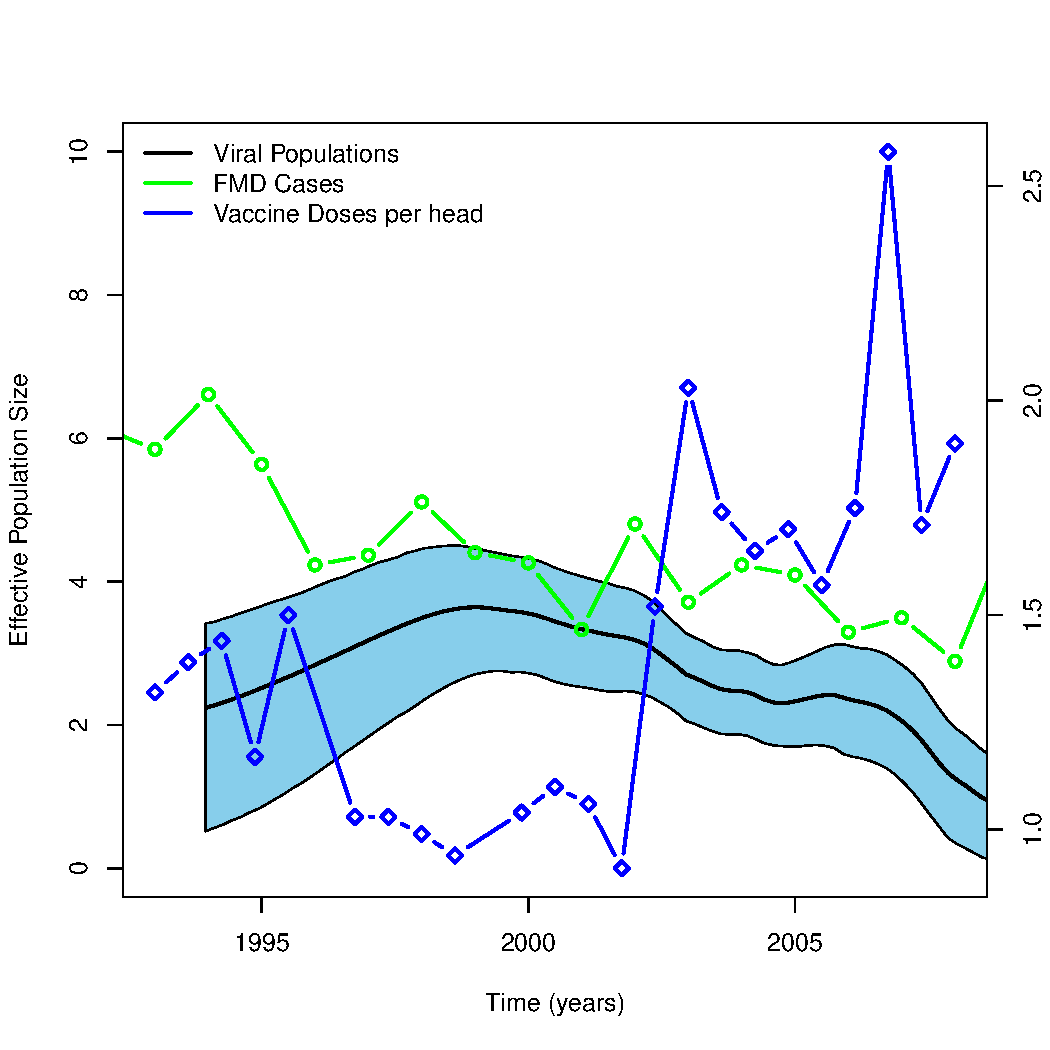
\includegraphics[scale=.60]{FIGURES/SFig_O2000sky.pdf}}
\end{center}
\caption{}
\label{sfig:only2000sky}
\end{figure}
%%%%%%%%%%%%%%%%
%%%%%%%%%%%%%%%%
\newpage
\begin{table}[H]
\caption{\textbf{Model selection using path sampling (PS) and stepping-stone sampling (SS) to determine the tree prior (coalescent) model and clock for both serotypes.}
UCLD = uncorrelated relaxed clock with an underlying log-normal distribution; UCED = uncorrelated relaxed clock with an underlying exponential distribution.
Best fitting models (highest log marginal likelihood obtained using SS) are highlighted in bold.
The more flexible non-parametric skyride tree prior clearly outperforms the assumption of a constant population size, which is consistent with the fact that FMDV (both serotypes) has experienced periods of population expansion, i.e. transmission within the time frame considered.
The assumption of a single rate for every lineage in the phylogeny is also rejected for both serotypes.
Remarkably, the best fitting relaxed clock models are different for each serotype, suggesting different branch (lineage) level heterogeneity levels between serotypes.
}
\begin{center}
\begin{tabular}{ccccccc}
\toprule
Serotype	& Coalescent	& Clock	& PS  & SS\\             
\midrule
A	& Constant	 & UCLD	& -12280.50& -12285.02\\
A	& Skyride 	& UCLD	& \textbf{-12273.68} & \textbf{-12274.59}\\
A	& Constant	 & UCED	& -12320.36 & -12316.16\\
A	& Skyride 	& UCED	& -12311.20 & -12307.87\\
A       & Skyride       & STRICT & -12315.31 & -12308.19\\
O	& Constant	& UCLD	& -8089.96& -8087.76\\
O	& Skyride 	& UCLD	& -8078.77 & -8082.64\\
O	& Constant	& UCED	&-8087.57 & -8090.10\\
O	& Skyride 	& UCED	& \textbf{-8064.67}& \textbf{-8069.47}\\
O       & Skyride       & STRICT & -8131.91& -8125.31\\
\bottomrule
\end{tabular}
\end{center}
\begin{flushleft}
\end{flushleft}
\label{stab:treeclockselection}
 \end{table}

%%%%%%%%%%%%%%%%
%%%%%%%%%%%%%%%%
\begin{table}[H]
 \caption{
 Representation of South American countries in the data sets analyzed.
 Full details (and accession numbers) are given in Text S1.
 From these summaries it's clear that some countries are over-represented in the data set.
 We provide a detailed sensitivity analysis to address the impact of this sample imbalance.
 }
 \begin{center}
 \begin{tabular}{cccc}
 \toprule
   \multicolumn{2}{c}{Serotype A}& \multicolumn{2}{c}{Serotype O}\\
 Country & number of sequences (time span)& number of sequences (time span) & \\ 
  \midrule
Argentina & $58$ ($1959$--$2001$)& $2$ ($2000$--$2006$)  \\
Bolivia   & $7$ ($2000$--$2001$)& $14$ ($2000$--$2002$)  \\
Brazil    & $16$ ($1955$--$2001$)& $15$ ($1998$--$2005$)  \\
Colombia  & $14$ ($1967$--$2008$)& $36$ ($1994$--$2008$)  \\
Ecuador   & $3$ ($1975$--$2002$)& $90$ ($2002$--$2010$)  \\
Paraguay                    & --& $2$ ($2002$--$2003$)  \\
Peru      & $4$ ($1969$--$2000$)& $1$ ($2004$)  \\
Uruguay   & $2$ ($2001$)& $1$ ($2000$)  \\
Venezuela & $27$ ($1962$--$2007$)& $6$ ($2003$--$2007$)  \\
Total     & $131$ ($1955$--$2008$) & $167$ ($1994$--$2010$)\\
  \bottomrule
 \end{tabular}
 \end{center}
\label{stab:reps}
\end{table}
 %%%%%%%%%%%%%%%%%%
 %%%%%%%%%%%%%%%%%%
\begin{sidewaystable}[h]
\caption{
\textbf{Spatial signal for FMDV serotypes A and O data sets.} 
We use Bayesian tip-association significance testing (BaTS) to assess the degree of spatial signal, measured as phylogeny-location association, contained in the posterior distribution of trees for both serotypes. 1-Monophyletic clade size
Overall, our results show that there is substantial location-phylogeny association, justifying richer phylogeographic analyses.}
\begin{tabular}{ccccccc}
\toprule
&\multicolumn{3}{c}{Serotype A} & \multicolumn{3}{c}{Serotype O} \\
MC$^1$ Statistic &Observed mean (95\% CI)&Null mean (95\% CI)&p-value &Observed mean (95\% CI)&Null mean (95\% CI)&p-value\\
\midrule
Argentina &12.31 (12.00, 14.00)	&3.45	(2.22, 5.11)	&0.001& 1.00 (1.00, 1.00)&	1.00 (1.00, 1.00)&	1.000\\
Brazil &10.27	(10.00, 11.00)	&2.02 (1.25, 3.00) &0.001& 19.00 (19.00, 19.00)&	2.19 (1.66, 3.03)&	0.001\\
Bolivia &6.00 (6.00, 6.00)	&1.39 (1.00, 2.00)	&0.001&1.00 (1.00, 1.00)&	1.00 (1.00, 1.00)&	1.000\\
Colombia &5.11 (5.00, 6.00)	&1.10  (1.00, 1.99)	&0.001&1.00 (1.00, 1.00)&	1.00 (1.00, 1.00)&	1.000\\
Ecuador &1.00 (1.00, 1.00)	&1.00 (1.00, 1.00)	&1.000&13.00 (13.00, 13.00)&	1.34 (1.00, 2.00)&	0.001\\
Paraguay&-- &-- &--  & 39.40 (31.00, 58.00)& 4.67 (3.43, 6.39)&0.001\\
Peru&1.00 (1.00, 1.00)	&1.02 (1.00, 1.00)&1.000&1.00 (1.00, 1.00)&1.01 (1.00, 1.00)&1.000\\
Uruguay &5.11 (5.00, 7.00)	&1.50	(1.00, 2.03)	&0.001&4.00 (4.00, 4.00)&	1.06 (1.00, 1.32)&	0.001\\
Venezuela&1.82 (1.00, 2.00)	&1.02 (1.00, 1.08)	&0.010&6.00 (6.00, 6.00)&	1.28 (1.00, 2.00)&	0.001\\
\bottomrule
\end{tabular}
\begin{flushleft}
\end{flushleft}
\label{stab:BaTS}
\end{sidewaystable}
%%%%%%%%%%%%%
%%%%%%%%%%%%%
\begin{table}[h]
\caption{ {{\bf Parameter estimation using the complete and without Argentina data sets for serotype A.}} 
To assess the impact of the over-representation of Argentina in our sample we remove all sequences from this location and re-estimate the parameters.
1- All 131 sequences were used. 2- Time to most recent common ancestor. 3- Codon positions $1$, $2$ and $3$.
Not surprisingly, the TMRCA estimated without Argentina is older, but note that the posterior CI's overlap.
These results show that the influence of Argentinian samples in the estimates is limited and over-representation does not pose an important problem for this analysis.}
\begin{center}
\begin{tabular}{ccc}
\toprule
Parameter	&Complete$^{1}$	& Without Argentina\\
\midrule
TMRCA$^{2}$	&76.40 (69.48-83.65)	&82.31 (72.40-92.81)\\
CP1$	^{3}$	&0.65 (0.54-0.76)	&0.62 (0.51-0.75)\\
CP2	&0.46 (0.37-0.58)	&0.41 (0.31-0.53)\\
CP3	&1.87 (1.74-2.00)	& 1.95 (1.81 -2.09)\\
Rate ($\times 10^{-3}$)	&4.14 (3.39-4.98)	&3.46 (2.82-4.11)\\
\bottomrule
\end{tabular}
\end{center}
\label{stab:SB_A}
 \end{table}
%%%%%%%%%
%%%%%%%%%
\begin{table}[h]
\caption{ {{\bf Parameter estimation using the complete and without Ecuador data sets for serotype O.}} 
To assess the impact of the overrepresentation of Ecuador (90 sequences) our sample we remove all sequence from this location and re-estimate the parameters.
1- All 167 sequences were used. 2- Time to most recent common ancestor. 3- Codon positions $1$, $2$ and $3$.
Similarly to what we found for serotype A, the results here suggest that the Ecuadorian sequences do not change the parameter estimates dramatically.}
\begin{center}
\begin{tabular}{ccc}
\toprule
Parameter	&Complete$^{1}$	&Without Ecuador\\
\midrule
TMRCA$^{2}$ & 21.25 (19.20-23.60) &22.65 (17.6-29.5)\\
CP1$^{3}$ & 0.51 (0.39-0.63) &0.51 (0.39-0.64)\\
CP2  &0.53 (0.39-0.69) & 0.42 (0.29-0.59)\\
CP3 &1.94 (1.78-2.10) & 2.05 (1.87 -2.21)\\
Rate ($\times 10^{-2}$)	&1.11 (0.91-1.32)&0.91 (0.63-1.21)\\
\bottomrule
\end{tabular}
\end{center}
\label{stab:SB_O}
 \end{table}

%%%%%%%%
%%%%%%%%
\newpage
\begin{sidewaystable}
\medskip
\begin{minipage}{\textwidth} 
\begin{center}
\caption{ {{\bf 'Equal down-sampling' experiment for serotype A.}} 
Five random down-sampled sub-samples were obtained and used for parameter inference.
1-- $\times 10^{-3}$; 2 -- $\times 10^{-2}$; 3-- Probability distribution at root node; 4-- Kullback-Leibler divergence (see Text).
It is clear that parameter estimates are consistent between sub-samples.
The estimation of the root state, however, is the exception.
The sub-sampled analyses show less concentrated posteriors (when compared with the full data) and one sub-sample yields a different root than was found for the other four. 
}
\begin{tabular}{cccccc}
\toprule
Sub-sample	&mean subs. rate$^{1}$ (95 \% BCI)	&TMRCA (95 \% BCI)	&mean migration rate$^{2}$  (95 \% BCI)	&Root (Pr$^{3}$)& KL$^4$\\
\midrule
1	&4.21 (3.43-5.05)	&78.97 (71.21-86.82)	&2.63 (1.34-4.08)	&Argentina (0.41)& 1.76\\
2	&4.25 (3.44-5.07)	&79.64 (71.49-88.04)	&2.54 (1.28-3.98)	&Brazil (0.40)& 1.41\\
3	&4.12 (3.38-4.94)	&77.74 (70.26-85-86)	&2.49 (1.27-3.88)	&Brazil (0.57)&1.47\\
4	&4.12 (3.41-4.82)	&77.60 (69.41-85.88)	&2.44 (1.21-3.85)	&Brazil (0.61)&0.98\\
5	&4.19 (3.49-4.93)	&78.28 (70.23-86.96)	&2.66 (1.31-4.11)	&Brazil (0.45)& 1.00\\
\bottomrule
\end{tabular}
\label{stab:ED_A}
\end{center}
\end{minipage}
\end{sidewaystable}

%%%%
%%%%
\newpage
\begin{sidewaystable}
\medskip
\begin{minipage}{\textwidth}
\begin{center}
 \caption{ {{\bf 'Equal down-sampling' experiment for serotype O.}} 
 Five random down-sampled sub-samples were obtained and used for parameter inference.
1-- $\times 10^{-3}$; 2--  Probability at root node; 3-- Kullback-Leibler divergence (see Text).
For serotype O both the parameter estimates and root location are in agreement between sub-samples, but likewise to serotype A, yield less concentrated posteriors (smaller KL divergences).}
\begin{tabular}{cccccc}
\toprule
Su-bsample	&mean subs. rate$^{1}$ (95 \% BCI)	&TMRCA (95 \% BCI)	&mean migration rate$^{1}$ (95 \% BCI)	&Root (Pr$^{2}$) & KL$^3$\\
\midrule
1	&1.11 (0.86-1.37)	&20.27 (18.45-21.95)	&8.48 (3.91-13.59)	&Venezuela  (0.45)& 1.24\\
2	&0.865 (0.62-1.11)	&22.40 (19.78-25.31)	&8.74 (3.84-14.28)	&Venezuela  (0.46)&1.04\\
3	&0.94 (0.68-1.21)	&21.91 (19.46-24.56)	&8.72 (4.03-14.17)	&Venezuela  (0.51)&1.52\\
4	&0.84 (0.62-1.18)	&22.54 (19.80-25.45)	&8.43 (3.77-13.67)	&Venezuela  (0.49)&1.00\\
5	&0.88 (0.63-1.13)	&22.33 (19.55-25.26)	&8.58 (3.89-13.18)	&Venezuela  (0.44)&1.23\\
\bottomrule
\end{tabular}
\label{stab:ED_O}
\end{center}
\end{minipage}
\end{sidewaystable}
%%%%
%%%%
\end{document}
